\documentclass{article}

\PassOptionsToPackage{numbers}{natbib}
\usepackage{neurips_2026}

\usepackage[utf8]{inputenc}
\usepackage[T1]{fontenc}
\usepackage{hyperref}
\usepackage{url}
\usepackage{booktabs}
\usepackage{amsfonts}
\usepackage{amsmath}
\usepackage{amssymb}
\usepackage{amsthm}
\usepackage{mathtools}
\usepackage{microtype}
\usepackage{xcolor}
\usepackage{graphicx}
\usepackage{subcaption}
\usepackage{bm}
\usepackage{tikz}
\usepackage{placeins}
\usetikzlibrary{arrows.meta,positioning}

\newtheorem{theorem}{Theorem}[section]
\newtheorem{proposition}[theorem]{Proposition}
\newtheorem{lemma}[theorem]{Lemma}
\newtheorem{corollary}[theorem]{Corollary}
\newtheorem{assumption}[theorem]{Assumption}
\newtheorem{definition}[theorem]{Definition}
\newtheorem{remark}[theorem]{Remark}

\newcommand{\R}{\mathbb{R}}
\newcommand{\N}{\mathbb{N}}
\newcommand{\E}{\mathbb{E}}
\newcommand{\Pp}{\mathbb{P}}
\newcommand{\one}{\mathbf{1}}
\newcommand{\calL}{\mathcal{L}}
\newcommand{\calF}{\mathcal{F}}
\newcommand{\calE}{\mathcal{E}}
\newcommand{\scrL}{\mathcal{L}}
\newcommand{\wh}{\widehat}
\newcommand{\llbracket}{[\![}
\newcommand{\rrbracket}{]\!]}
\DeclareMathOperator{\rank}{rank}
\DeclareMathOperator{\im}{Im}
\DeclareMathOperator*{\argmin}{arg\,min}

\title{Global Convergence and Better Spectral Bias in Low-Rank Neural Networks}

\author{Anonymous Authors}

\begin{document}

\maketitle

\begin{abstract}
Neural networks often struggle to learn highly oscillatory functions at finite training time: low-frequency components are fitted first, while high-frequency modes can remain poorly recovered even when the model is expressive enough to represent them. Low-rank networks are usually introduced as compressed alternatives to dense models, but this view overlooks a more useful possibility: rank can act as a structural control on what the network learns first. In this paper, we show that this is the case. We first prove that low-rank random-feature networks in the mean-field limit converge to a global minimizer of the population risk whenever their limiting dynamics converge. We then show that the rank is not merely a compression parameter: choosing it correctly can reduce the number of trainable degrees of freedom while also improving the fit of highly oscillatory targets. The key practical message is that the best rank is typically intermediate. If the rank is too small, the model lacks expressivity; if it is too large, it recovers the finite-time bias of the dense model. Controlled geometric and Fourier diagnostics, together with high-frequency regression experiments, show that an appropriate low rank can lower test loss, improve high-frequency recovery, and that the optimal rank shifts with the target spectrum and training objective.
\end{abstract}

\section{Introduction}
\label{sec:introduction}

This section states the main problem, explains why low rank is more than compression, and summarizes the convergence and spectral-bias contributions.

Low-rank neural networks replace dense matrices by factored or bottlenecked operators. The standard motivation is computational: fewer trainable parameters and cheaper memory traffic. This paper argues that the more important question is mathematical. Can rank be used as a principled control on training dynamics rather than only as a compression parameter?

This question is important for scientific machine learning. Many tasks in AI for science require learning functions with oscillations, sharp transitions, multiscale structure, or high-frequency Fourier content: wave fields, PDE solution operators, molecular potentials, turbulent signals, and inverse problems all contain information at small spatial or temporal scales. Neural networks can represent such functions, but finite-time training often learns smooth, low-frequency components first. This frequency bias can be modified by the data distribution or by replacing the loss with a Sobolev norm~\cite{yu2022tuning}; our question is whether the architecture itself, through rank, can provide another control parameter. This makes the problem difficult: expressivity alone is not enough, and a model that is globally trainable in principle can still fail to recover the high-frequency part under a realistic training budget.

We answer the first question positively for a low-rank random-feature architecture. The model freezes a rich random-feature map and trains low-rank channel weights through mean-field gradient flow. Since the frozen features keep a dense span throughout training, the usual obstruction in deep mean-field convergence proofs is removed: at a limit point, zero gradient implies the conditional first-order condition for the loss, and the loss-identifiability assumption forces global optimality. Low rank enters through the mixing matrix and channel index, changing constants but not the logic of the proof.

The second question is more subtle. Global convergence is an asymptotic statement: it says what happens if the population dynamics settle. Spectral bias is a finite-time phenomenon: it asks which parts of the target are reached first under a limited optimization budget. These two views can disagree on oscillatory targets, because a model may be globally trainable and still spend most of training on the low-frequency part of the signal. We show that rank changes this finite-budget behavior by changing the geometry of ReLU networks, hence which Fourier modes are recovered early. The practical outcome is a rank-selection rule: choose the smallest rank that avoids the approximation bottleneck while improving high-frequency recovery.

\paragraph{Contributions.}
The paper makes three contributions:
\begin{itemize}
\item We give a globally convergent anchor model for low-rank networks. Freezing a rich random-feature map keeps the feature span from collapsing, while the trainable low-rank channels still allow a mean-field feature-learning interpretation.
\item We explain why rank can change high-frequency learning. In ReLU networks, lowering rank reduces the number of independent path constraints, which changes the piecewise-affine geometry that controls Fourier energy.
\item We provide controlled diagnostics for choosing rank. The experiments show that the useful rank is usually intermediate and moves with the target spectrum or training objective, so rank should be selected from spectral recovery rather than parameter count alone.
\end{itemize}

\section{Related Work}
\label{sec:related}

This section positions the paper relative to mean-field convergence, low-rank adaptation, bottleneck-rank theory, and spectral bias.

\paragraph{Mean-field convergence.}
Mean-field theory analyzes neural network training through the deterministic evolution of parameter distributions in the large-width limit. Foundational work established global convergence mechanisms for two-layer models and Wasserstein gradient flows under suitable convexity, homogeneity, or support assumptions~\cite{mei2018,chizat2018}. Later multilayer mean-field analyses clarified how deep feature maps evolve and when stationary points can be related to global optima~\cite{pham2021,nguyen2023}. Our result follows this line but focuses on low-rank random-feature networks: the existence and uniqueness estimates use the same mean-field template, while the convergence proof must be adapted to channel-wise low-rank couplings.

\paragraph{Low-rank and random features.}
Low-rank neural networks are often motivated by parameter efficiency, with LoRA-style decompositions now standard in large-scale adaptation~\cite{hu2021}. Recent theory has begun to explain why LoRA can be trainable: Jang, Lee, and Ryu~\cite{jang2024lora} show that, in the NTK fine-tuning regime, sufficiently large LoRA rank removes spurious local minima and yields low-rank solutions with good generalization. Most theory for low-rank networks focuses on expressivity, approximation, kernel behavior, or LoRA fine-tuning rather than global mean-field training dynamics. Random features provide a tractable bridge between finite networks and kernel methods: fixing the feature map turns the representation into a stable basis, while training the channel weights retains a mean-field optimization problem. In our RF-LR setting, frozen random features prevent support collapse and preserve the dense-span property needed for the stationarity-to-optimality argument; the low-rank factors enter through bounded channel mixing rather than through a full dense contraction chain.

\begin{figure}[t]
\centering
\resizebox{0.68\textwidth}{!}{%
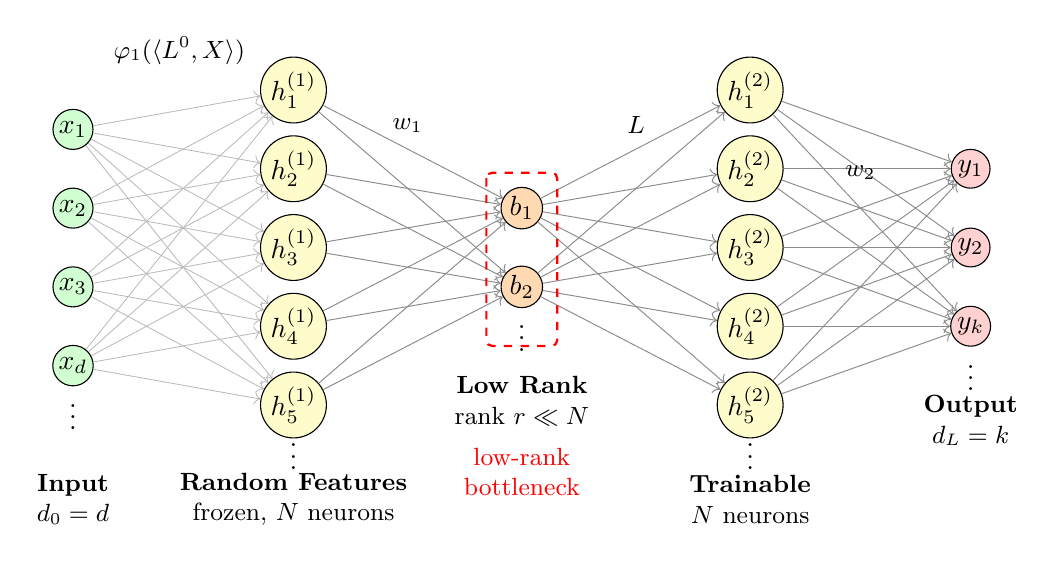
\begin{tikzpicture}[
    neuron/.style={circle, draw, fill=blue!15, minimum size=13pt, inner sep=1pt},
    input/.style={circle, draw, fill=green!18, minimum size=13pt, inner sep=1pt},
    output/.style={circle, draw, fill=red!18, minimum size=13pt, inner sep=1pt},
    hidden/.style={circle, draw, fill=yellow!20, minimum size=13pt, inner sep=1pt},
    bottleneck/.style={circle, draw, fill=orange!30, minimum size=13pt, inner sep=1pt},
    conn/.style={->, draw=black!45, line width=0.35pt},
    frozenconn/.style={->, draw=gray!55, line width=0.3pt},
    lab/.style={font=\small, align=center}
]
\node[input] (x1) at (0,2) {$x_1$};
\node[input] (x2) at (0,1) {$x_2$};
\node[input] (x3) at (0,0) {$x_3$};
\node[input] (xd) at (0,-1) {$x_d$};
\node at (0,-1.55) {$\vdots$};

\node[hidden] (h11) at (2.8,2.5) {$h_1^{(1)}$};
\node[hidden] (h12) at (2.8,1.5) {$h_2^{(1)}$};
\node[hidden] (h13) at (2.8,0.5) {$h_3^{(1)}$};
\node[hidden] (h14) at (2.8,-0.5) {$h_4^{(1)}$};
\node[hidden] (h15) at (2.8,-1.5) {$h_5^{(1)}$};
\node at (2.8,-2.05) {$\vdots$};

\node[bottleneck] (b1) at (5.7,1) {$b_1$};
\node[bottleneck] (b2) at (5.7,0) {$b_2$};
\node at (5.7,-0.55) {$\vdots$};

\node[hidden] (h21) at (8.6,2.5) {$h_1^{(2)}$};
\node[hidden] (h22) at (8.6,1.5) {$h_2^{(2)}$};
\node[hidden] (h23) at (8.6,0.5) {$h_3^{(2)}$};
\node[hidden] (h24) at (8.6,-0.5) {$h_4^{(2)}$};
\node[hidden] (h25) at (8.6,-1.5) {$h_5^{(2)}$};
\node at (8.6,-2.05) {$\vdots$};

\node[output] (y1) at (11.4,1.5) {$y_1$};
\node[output] (y2) at (11.4,0.5) {$y_2$};
\node[output] (yk) at (11.4,-0.5) {$y_k$};
\node at (11.4,-1.05) {$\vdots$};

\foreach \i in {1,2,3,d} {
    \foreach \j in {11,12,13,14,15} {
        \draw[frozenconn] (x\i) -- (h\j);
    }
}
\foreach \i in {11,12,13,14,15} {
    \foreach \j in {1,2} {
        \draw[conn] (h\i) -- (b\j);
    }
}
\foreach \i in {1,2} {
    \foreach \j in {21,22,23,24,25} {
        \draw[conn] (b\i) -- (h\j);
    }
}
\foreach \i in {21,22,23,24,25} {
    \foreach \j in {1,2,k} {
        \draw[conn] (h\i) -- (y\j);
    }
}

\node[lab] at (0,-2.7) {\textbf{Input}\\$d_0=d$};
\node[lab] at (2.8,-2.7) {\textbf{Random Features}\\frozen, $N$ neurons};
\node[lab] at (5.7,-1.45) {\textbf{Low Rank}\\rank $r\ll N$};
\node[lab] at (8.6,-2.7) {\textbf{Trainable}\\$N$ neurons};
\node[lab] at (11.4,-1.7) {\textbf{Output}\\$d_L=k$};

\node[font=\small] at (1.35,3) {$\varphi_1(\langle L^0,X\rangle)$};
\node[font=\small] at (4.25,2.05) {$w_1$};
\node[font=\small] at (7.15,2.05) {$L$};
\node[font=\small] at (10.0,1.45) {$w_2$};

\draw[red, thick, dashed, rounded corners=2pt] (5.25,1.45) rectangle (6.15,-0.75);
\node[red, font=\small, align=center] at (5.7,-2.35) {low-rank\\bottleneck};
\end{tikzpicture}%
}
\caption{Architecture of a three-layer low-rank random-feature network with frozen random features, a rank-$r$ bottleneck, and trainable output weights.}
\label{fig:architecture}
\end{figure}

\paragraph{Bottleneck rank and implicit low-rank bias.}
Recent work gives a functional notion of optimal rank that is closer to our setting than the algebraic rank of a single matrix. Jacot~\cite{jacot2022implicitrank} studies the implicit bias of large-depth homogeneous networks and shows that their representation cost converges toward a nonlinear rank notion, sandwiched between Jacobian rank and bottleneck rank. The bottleneck rank is the smallest inner dimension $k$ for which a function can be factored as $f=h\circ g$ through $\R^k$. Follow-up work~\cite{jacot2023bottleneck} proves that learned deep representations exhibit a bottleneck structure and introduces finite-depth corrections that balance low inner dimension against regularity. This suggests a theoretical target rank: the smallest rank that captures the intrinsic bottleneck dimension of the target without forcing an irregular or rank-underestimating interpolant. Complementarily, Bantzis, Simon, and Jacot~\cite{bantzis2025saddle} show that the first saddle escape of deep ReLU networks has a low-rank bias in deeper layers and propose saddle-to-saddle dynamics with increasing bottleneck rank. Our rank-selection principle is consistent with this picture: training should start from low effective rank, but useful learning requires increasing rank until approximation and spectral recovery saturate.

\paragraph{Spectral bias.}
The spectral-bias literature identifies why neural networks often fit low-frequency components before high-frequency components. Rahaman et al.~\cite{rahaman2019} connect this learning order to Fourier properties of piecewise linear networks, while Yu, Yang, and Townsend~\cite{yu2022tuning} show that the bias can be tuned through nonuniform data and Sobolev-type losses. This paper keeps that Fourier viewpoint but changes the intervention: instead of reweighting data or losses, we study rank as an architectural parameter that changes the geometry seen by finite-time training.

\section{Freezing Half the Weights Allows Global Convergence}
\label{sec:model}

This section defines the RF-LR mean-field model and states the conditional global convergence theorem.

Let $X\in\R^d$ and $Y$ be drawn from a population distribution. The finite-width low-rank random-feature network used throughout the paper is the one from the original experiments:
\begin{equation}
h^{(0)}(x)=x,\qquad
h^{(\ell)}(x)=
\frac1{n_\ell}\sum_{j=1}^{n_\ell}
w_j^{(\ell)}
\varphi_\ell\!\left(
\langle L_j^{(\ell)},h^{(\ell-1)}(x)\rangle+b_j^{(\ell)}
\right),
\label{eq:finite-rflr}
\end{equation}
where the feature directions $L_j^{(\ell)}$ and biases $b_j^{(\ell)}$ are frozen, while the channel weights $w_j^{(\ell)}$ are trained. This is a low-rank factorization of a dense layer in which the left factor is fixed: if $W_\ell=U_\ell V_\ell^\top$ with $U_\ell\in\R^{n_\ell\times r_\ell}$ bounded and full column rank, then $U_\ell$ plays the role of a frozen random-feature or mixing basis and the trainable factor $V_\ell$ is absorbed into the channel weights. Thus one may avoid training $U_\ell$ entirely; drawing it as a bounded full-rank tall-skinny matrix is enough for the theory, while choosing $U_\ell\in\mathrm{St}(n_\ell,r_\ell)$ is an optional numerical normalization.

\subsection{Mean-Field Formulation}

The mean-field viewpoint is the relevant one for global convergence. Pure kernel or neural-tangent analyses give convexity by freezing the representation, but they largely remove feature learning. Finite-width nonconvex analyses allow feature learning but rarely provide global convergence guarantees for deep low-rank networks. Mean-field theory is currently the most developed framework that can keep a feature-learning interpretation while still proving that limiting gradient-flow trajectories reach global minimizers under identifiability assumptions. We use a frozen-feature low-rank specialization because it is the cleanest setting in which the dense-span argument is preserved; it should be viewed as the globally convergent anchor case for more general low-rank feature-learning models.

In the mean-field limit, frozen feature maps are written $L^0(C_\ell)$ and trainable channel weights are written $w_\ell(t,C_\ell)$. The channel mixer $L\in\R^{N_2\times r}$ is a bounded full-column-rank tall-skinny factor, not necessarily an orthogonal matrix. We write the second-layer operator as $W_2=L A_2^\top$, with $L$ fixed and $A_2$ trainable, then absorb the small right factor $A_2^\top$ into the rank-channel functions below. One may additionally choose $L\in\mathrm{St}(N_2,r)$, or periodically re-orthogonalize it, as a numerical design choice; this is natural for matrix-structured optimizers such as Muon, which orthogonalize matrix updates by Newton--Schulz or polar iterations~\cite{jordan2024muon,boreiko2025muon}. In the two-hidden-layer case, the first partial functions are
\begin{equation}
f_k(t,x)=\E_{C_1}\left[w_1(t,C_1,k)\,\varphi_1\left(\langle L^0(C_1),x\rangle\right)\right],
\qquad k=1,\ldots,r,
\end{equation}
and the second-layer preactivation is
\begin{equation}
H_2(t,c_2;x)=\sum_{k=1}^r L_{c_2,k} f_k(t,x).
\end{equation}
Thus $H_2$ is the reconstruction of the second-layer signal from a bounded rank-$r$ channel basis. The output is obtained by averaging the trainable top weights against $\varphi_2(H_2)$. For deeper networks, the same alternating pattern is used: trainable channel weights are averaged against frozen random features and mixed through bounded low-rank channel matrices.

The population objective is
\begin{equation}
\scrL(W)=\E_{(X,Y)}\left[\calL\left(Y,\hat y(X;W)\right)\right].
\end{equation}
The mean-field gradient flow evolves the trainable weights by
\begin{equation}
\partial_t w_\ell(t,\cdot)=-\xi_\ell(t)\,\nabla_{w_\ell}\scrL(W(t)),
\label{eq:generic-flow}
\end{equation}
where $\xi_\ell$ are bounded learning-rate schedules. The exact formulas are standard backpropagation in the mean-field variables; the only low-rank modification is the channel mixing through $L_{c_\ell,k}$.

Under the technical regularity, diversity, loss-identifiability, and convergence assumptions stated in Appendix~\ref{app:assumptions}, freezing the feature directions gives a well-defined mean-field system and allows the usual stationarity argument to conclude global optimality.

\begin{theorem}[Well-posedness and conditional global convergence of RF-LR training]
\label{thm:convergence}
Under Assumptions~\ref{assump:regularity}--\ref{assump:convergence}, the low-rank mean-field gradient-flow system has a unique solution on every finite interval $[0,T]$ and therefore on $[0,\infty)$. Moreover, if the resulting low-rank mean-field dynamics converges to $W^\star$ in the modified $\mathcal W_4$ coupling topology defined in Appendix~\ref{app:assumptions} through Assumption~\ref{assump:convergence}, then $W^\star$ is a global minimizer of the population loss:
\begin{equation}
\scrL(W^\star)=\inf_W \scrL(W).
\end{equation}
For every depth $L\ge2$, this holds with standard independent initialization of the trainable weights.
\end{theorem}

The convergence statement is conditional: as in the corresponding multilayer mean-field results, we do not prove that every trajectory converges. The theorem says that convergence cannot occur to a bad stationary point under the stated dense-span, non-degeneracy, and loss-identifiability assumptions. The well-posedness part only justifies that the limiting dynamics are genuine ODEs rather than formal flows. This is the natural Picard argument of Nguyen and Pham~\cite{nguyen2023}: nothing structural changes in the proof, except that dense-layer operator norms are replaced by bounded low-rank mixing constants. The complete well-posedness proof is deferred to the supplementary material, Appendix~\ref{app:wellposed-proof}.

\begin{proof}[Proof idea]
The existence and uniqueness part follows the standard mean-field fixed-point argument, whose full details are given in Appendix~\ref{app:wellposed-proof}. We only summarize the convergence-to-global-minimum step here; Appendix~\ref{app:global-proof} gives the full notation and the five formal steps. We assume that gradient descent, or its mean-field gradient-flow limit, has converged somewhere: $W(t)\to\bar W$ in the modified $\mathcal W_4$ coupling topology defined in Appendix~\ref{app:assumptions}. Stationarity and the persistent dense span of the frozen first-layer features then imply the integrated identity
\begin{equation}
\E\!\left[
d_L(Z;\bar W)\,B_k^{(2)}(X;\bar W)
\mid X=x
\right]=0
\quad\text{for }\Pp_X\text{-a.e. }x,\quad k=1,\ldots,r,
\label{eq:proofidea-dense-product}
\end{equation}
where $d_L(Z;\bar W)=\partial_2\calL(Y,\hat y(X;\bar W))$ and $B_k^{(2)}$ is the channel-wise backpropagated factor defined in Appendix~\ref{app:global-proof}.

\emph{Step 3: remove the backpropagated factor.}
The non-degeneracy assumptions exclude a dead-channel limit: for $\Pp_X$-a.e. $x$, at least one channel has a nonzero backpropagated factor $B_k^{(2)}(x;\bar W)$. The identity we use keeps this factor inside the conditional expectation:
\[
\E\!\left[
d_L(Z;\bar W)B_k^{(2)}(X;\bar W)
\mid X=x
\right]=0
\quad\text{for }\Pp_X\text{-a.e. }x,\quad k=1,\ldots,r.
\]
Since $B_k^{(2)}(X;\bar W)$ is $X$-measurable, the non-degeneracy assumption then allows us to choose at least one nonzero backpropagated factor at almost every $x$, so
\begin{equation}
\E\!\left[
\partial_2\calL\left(Y,\hat y(X;\bar W)\right)
\mid X=x
\right]=0
\quad\text{for }\Pp_X\text{-a.e. }x.
\label{eq:proofidea-conditional-zero}
\end{equation}

\emph{Step 5: the trajectory loss converges to the limit loss.}
Since $W(t)\to\bar W$ in the modified $\mathcal W_4$ coupling topology defined in Appendix~\ref{app:assumptions}, there are couplings $\pi_t$ between $W(t)$ and $\bar W$ whose weighted channel gaps vanish. In the two-layer channel notation, the key convergence statement is exactly
\begin{equation}
\E_{\pi_t}\!\left[(1+|\bar w_2|)|\bar w_2|
\sum_{k=1}^r |\bar w_{1,k}|\,|w_{1,k}-\bar w_{1,k}|\right]\to0,
\end{equation}
with analogous quantities for all deeper layers. The forward stability estimate uses the ReLU channel expansion of a low-rank preactivation,
\begin{equation}
\left|\operatorname{ReLU}\!\left(\sum_{k=1}^r x_k\right)
-\operatorname{ReLU}\!\left(\sum_{k=1}^r y_k\right)\right|
\le \sum_{k=1}^r |x_k-y_k|.
\label{eq:proofidea-relu-channel}
\end{equation}
Together with the low-rank form $H_2=\sum_k L_{c_2,k}f_k$, \eqref{eq:proofidea-relu-channel} bounds every forward and backward difference by the same channel integrals. Hence
\begin{equation}
\E\left[
\left|\hat y(X;W(t))-\hat y(X;\bar W)\right|
\right]\to0.
\end{equation}
Lipschitzness of the loss in its second argument on the a priori bounded trajectory yields
\begin{equation}
|\scrL(W(t))-\scrL(\bar W)|
\le
K\,\E\left[
\left|\hat y(X;W(t))-\hat y(X;\bar W)\right|
\right]\to0.
\end{equation}

\emph{Step 4: identify the limit as globally optimal.}
By the loss-identifiability condition in Assumption~\ref{assump:loss}, namely \eqref{eq:loss-identifiability} in Appendix~\ref{app:assumptions},
\begin{equation}
\E[\partial_2\calL(Y,u)\mid X=x]=0
\quad\Longrightarrow\quad
\E[\calL(Y,u)\mid X=x]=0.
\end{equation}
Applying this with $u=\hat y(x;\bar W)$ and using non-negativity of $\calL$ gives
\begin{equation}
\scrL(\bar W)=0=\inf_W \scrL(W).
\end{equation}
Together with Step 5, $\scrL(W(t))\to\scrL(\bar W)$.
\end{proof}

\section{Low-Rank Spectral Bias}
\label{sec:spectral-transition}

This section explains how low-rank path constraints change CPWL geometry and the Fourier coefficients that control finite-resolution spectral bias.

\paragraph{Connection to spectral bias.}
Theorem~\ref{thm:convergence} says that a convergent trajectory reaches a global minimizer, but it does not describe the order in which Fourier modes are recovered at finite time. This section explains the architectural mechanism behind that order: low rank constrains active path coefficients and switching geometry, so it changes the CPWL face moments that control finite-resolution Fourier transfer. Thus the role of Rahaman et al.~\cite{rahaman2019} here is not only as prior related work, but as the Fourier template that our rank-dependent face-moment calculation refines.

In a ReLU network, on every activation region the network is affine, and the affine coefficient is a sum over active paths. We use the same path-product viewpoint as in path-based analyses of loss surfaces and finite-width neural kernels~\cite{choromanska2015,hanin2019finite}. For a scalar-output depth-$L$ network, this can be written schematically as
\begin{equation}
f(x)=
\sum_{p=(i_0,\ldots,i_L)}
\left(
\prod_{\ell=1}^{L} W^{(\ell)}_{i_\ell i_{\ell-1}}
\right)
\left(
\prod_{\ell=1}^{L-1}\mathbf 1_{\{h^{(\ell)}_{i_\ell}(x)>0\}}
\right)
x_{i_0},
\label{eq:path-expansion}
\end{equation}
where $p$ ranges over input-to-output paths. If $W_\ell=U_\ell V_\ell^\top$ has rank $r_\ell$, then many symbolic paths share the same latent channels, so their coefficients cannot vary independently. These path constraints also constrain ReLU switching normals $\nabla_x h^{(\ell)}_j(x)$: the normals lie in a smaller span than in a dense layer. Geometrically, this suppresses low-dimensional, high-codimension intersections; spectrally, the Fourier shell law below predicts more visible facet-dominated high-frequency mass.

\paragraph{Mechanism summary.}
Figure~\ref{fig:mechanism-summary} summarizes the mechanism. A low-rank factorization reduces independent path coefficients in \eqref{eq:path-expansion}; this constrains switching normals, suppresses high-codimension CPWL faces, and moves shell-averaged Fourier energy toward the facet-dominated regime of Rahaman et al.~\cite{rahaman2019}. The useful rank is intermediate: too small gives approximation error, while too large recovers the full-rank low-frequency-first bias. A frequency shell means modes with comparable radius $\|\xi\|\simeq\rho$.

\begin{figure}[t]
\centering
\resizebox{\textwidth}{!}{%
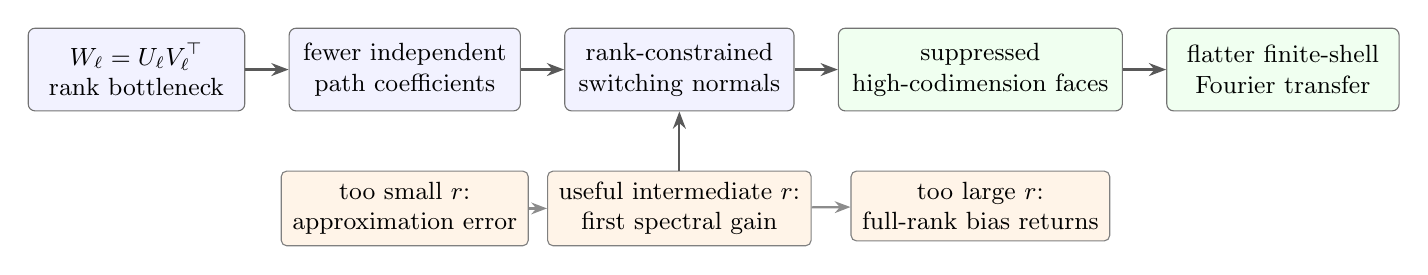
\begin{tikzpicture}[
    font=\small,
    box/.style={
        draw=black!55,
        rounded corners=2.5pt,
        align=center,
        minimum width=2.75cm,
        minimum height=1.05cm,
        inner sep=5pt,
        fill=blue!5
    },
    effect/.style={
        draw=black!55,
        rounded corners=2.5pt,
        align=center,
        minimum width=2.95cm,
        minimum height=1.05cm,
        inner sep=5pt,
        fill=green!6
    },
    warning/.style={
        draw=black!50,
        rounded corners=2pt,
        align=center,
        minimum width=3.1cm,
        minimum height=0.72cm,
        inner sep=4pt,
        fill=orange!9
    },
    arrow/.style={-{Stealth[length=2.2mm]}, thick, draw=black!65}
]
\node[box] (factor) {$W_\ell=U_\ell V_\ell^\top$\\rank bottleneck};
\node[box, right=0.55cm of factor] (paths) {fewer independent\\path coefficients};
\node[box, right=0.55cm of paths] (normals) {rank-constrained\\switching normals};
\node[effect, right=0.55cm of normals] (faces) {suppressed\\high-codimension faces};
\node[effect, right=0.55cm of faces] (fourier) {flatter finite-shell\\Fourier transfer};

\draw[arrow] (factor) -- (paths);
\draw[arrow] (paths) -- (normals);
\draw[arrow] (normals) -- (faces);
\draw[arrow] (faces) -- (fourier);

\node[warning, below=0.75cm of paths] (smallrank) {too small $r$:\\approximation error};
\node[warning, below=0.75cm of normals] (usefulrank) {useful intermediate $r$:\\first spectral gain};
\node[warning, below=0.75cm of faces] (largerank) {too large $r$:\\full-rank bias returns};

\draw[arrow] (usefulrank) -- (normals);
\draw[-{Stealth[length=2.0mm]}, thick, draw=black!45] (smallrank) -- (usefulrank);
\draw[-{Stealth[length=2.0mm]}, thick, draw=black!45] (usefulrank) -- (largerank);
\end{tikzpicture}%
}
\caption{Mechanism summary linking low-rank factorization, path coefficients, switching normals, CPWL faces, and finite-shell Fourier transfer.}
\label{fig:mechanism-summary}
\end{figure}

This connects to bottleneck rank: the population lower bound is the smallest inner dimension through which the target can factor~\cite{jacot2022implicitrank,jacot2023bottleneck}, while the finite-budget choice also balances optimization and spectral recovery. In experiments, we estimate this by the first rank where approximation is controlled and Fourier recovery no longer improves.

This algebraic constraint becomes geometric. Inside a cell of the previous layers, a new switching normal has the form
\begin{equation}
n_{\ell i\varepsilon}=B_{\ell-1,\varepsilon}^{\top}V_\ell u_{\ell i}
\in \im(B_{\ell-1,\varepsilon}^{\top}V_\ell),
\qquad
\dim \im(B_{\ell-1,\varepsilon}^{\top}V_\ell)\le \min(d,r_1,\ldots,r_\ell).
\end{equation}
Thus rank lowers the dimension of the normal subspace and suppresses high-codimension faces first.

\paragraph{Face Fourier expansion.}
Let $g=\chi f$, where $f$ is CPWL on a finite polyhedral complex in $\R^d$ and $\chi\in C_c^\infty(\R^d)$ is an observation window. Let $\mathcal F_q(f)$ be the codimension-$q$ faces of the complex. For every large frequency $\xi=\rho\theta$, $\theta\in\mathbb S^{d-1}$, the Fourier transform has the expansion
\begin{equation}
\wh g(\rho\theta)
=
\sum_{q=1}^d
\rho^{-(q+1)}
\sum_{F\in\mathcal F_q(f)}
A_F(\rho,\theta)
+O(\rho^{-(d+2)}),
\label{eq:face-expansion}
\end{equation}
where $A_F$ is a bounded oscillatory face coefficient controlled by the jump $\Delta_F$ of the appropriate normal derivative across the local fan around $F$. In particular,
\begin{equation}
|A_F(\rho,\theta)|
\le C_\chi \|\Delta_F\|\,\operatorname{vol}_{d-q}(F)\,\omega_F(\theta).
\end{equation}
This is the anisotropic phenomenon isolated by Rahaman et al.~\citep{rahaman2019}: in almost all directions a ReLU network has fast $k^{-(d+1)}$ amplitude decay, while in special directions orthogonal to facets of the linear regions the decay can be as slow as $k^{-2}$. Thus low codimension faces are precisely the geometric structures that keep high-frequency Fourier mass visible at finite resolution.

\begin{proposition}[Fourier shell law for CPWL networks]
\label{prop:shell-law}
Let $g=\chi f$ be a windowed continuous piecewise affine network in dimension $d$. Define the codimension-$q$ face moment
\begin{equation}
M_q(f)=
\sum_{F\in\mathcal F_q(f)}
\|\Delta_F\|^2
\operatorname{vol}_{d-q}(F)^2
\E_{\theta\in\mathbb S^{d-1}}\omega_F(\theta)^2 .
\end{equation}
Then the shell-averaged Fourier energy satisfies
\begin{equation}
S_f(\rho)=\E_{\|\xi\|\simeq \rho}|\wh g(\xi)|^2
\lesssim
\sum_{q=1}^d M_q(f)\rho^{-2(q+1)}.
\label{eq:shell-law}
\end{equation}
Low rank suppresses $M_q$ for larger $q$ first, moving finite-resolution spectra toward the facet-dominated $\rho^{-4}$ energy regime. This should be read as a coefficient statement rather than a claim that low rank creates a new universal exponent: the useful comparison with full rank is the reduction of $M_q/M_1$ and of the transition coefficient $(M_q/M_1)\rho^{-2q+2}$ for $q\ge2$.
\end{proposition}

\begin{proof}[Proof idea]
Write $f$ on its polyhedral complex as an affine function on each cell and set $g=\chi f$ with a smooth compactly supported window. The Fourier transform is then a sum of ordinary oscillatory integrals over cells. Integrating by parts in the direction $\theta=\xi/\|\xi\|$ produces boundary terms on cell facets. The order-$\rho^{-1}$ traces cancel across interior facets because the CPWL network is continuous and the same window multiplies both sides.

The first non-canceling term is therefore the jump of the directional derivative across a facet, hence it carries the factor $\rho^{-2}$. Repeating the same integration-by-parts argument on the induced face complex localizes the next non-smooth terms on codimension-$q$ faces, with amplitude order $\rho^{-(q+1)}$. This gives the face expansion \eqref{eq:face-expansion}, with coefficients controlled by the corresponding normal-derivative jumps and face volumes. This is the same anisotropic mechanism emphasized by Rahaman et al.~\citep{rahaman2019}: generic directions decay quickly, while directions close to facet normals can retain slow $|\xi|^{-2}$ amplitude decay.

Squaring the expansion and averaging over a frequency shell gives diagonal face energies of order $M_q(f)\rho^{-2(q+1)}$. Oscillatory cross terms are either lower order by angular non-stationary phase or absorbed into the same moments by Cauchy--Schwarz. Thus the exponent is determined by codimension, while rank changes the coefficients $M_q(f)$ by suppressing high-codimension intersections. A detailed integration-by-parts proof is given in Appendix~\ref{app:cpwl-proof}.
\end{proof}

\iffalse
Write the CPWL network on its polyhedral complex as
\begin{equation}
f(x)=\sum_{\varepsilon}
(a_\varepsilon^\top x+b_\varepsilon)\mathbf 1_{P_\varepsilon}(x),
\qquad
g(x)=\chi(x)f(x).
\end{equation}
The cutoff makes $g$ compactly supported, so
\begin{equation}
\wh g(\rho\theta)
=
\sum_\varepsilon
\int_{P_\varepsilon}
e^{-i\rho\langle \theta,x\rangle}
\chi(x)(a_\varepsilon^\top x+b_\varepsilon)\,dx
\end{equation}
is an ordinary oscillatory integral. Set $D_\theta=\theta\cdot\nabla$. Since
$D_\theta e^{-i\rho\langle\theta,x\rangle}=-i\rho e^{-i\rho\langle\theta,x\rangle}$,
the divergence theorem on each cell gives
\begin{align}
\int_{P_\varepsilon}e^{-i\rho\langle\theta,x\rangle}u_\varepsilon(x)\,dx
&=
\frac{i}{\rho}
\int_{\partial P_\varepsilon}
e^{-i\rho\langle\theta,x\rangle}
u_\varepsilon(x)\langle\theta,n_\varepsilon(x)\rangle\,d\sigma(x)
\nonumber\\
&\quad
-
\frac{i}{\rho}
\int_{P_\varepsilon}
e^{-i\rho\langle\theta,x\rangle}
D_\theta u_\varepsilon(x)\,dx,
\label{eq:first-ibp-cell}
\end{align}
where $u_\varepsilon(x)=\chi(x)(a_\varepsilon^\top x+b_\varepsilon)$ and
$n_\varepsilon$ is the outward normal. When the boundary terms are summed over all cells, every interior facet $F=P_\varepsilon\cap P_{\varepsilon'}$ is counted twice with opposite normals. The order-$\rho^{-1}$ trace contribution is therefore proportional to
\begin{equation}
\left(u_\varepsilon|_F-u_{\varepsilon'}|_F\right)
\langle \theta,n_F\rangle .
\end{equation}
Because $f$ is continuous and the same smooth window $\chi$ multiplies both traces, this term vanishes on internal facets. Boundary terms on the exterior of the observation window are smooth cutoff terms and can be integrated by parts arbitrarily many times, hence are absorbed in the final remainder.

After this cancellation, the leading non-smooth contribution comes from applying the same identity to the interior integral involving $D_\theta u_\varepsilon$. On a facet $F$ shared by two cells, its jump is
\begin{equation}
\big[D_\theta u\big]_F
=
\chi\,\theta^\top(a_\varepsilon-a_{\varepsilon'})
\end{equation}
because the terms involving derivatives of $\chi$ multiply the continuous trace of $f$ and cancel across $F$. Thus the first non-canceling boundary term is a jump of directional derivatives, and it carries the factor $\rho^{-2}$. This gives the codimension-one part of \eqref{eq:face-expansion}. In the special directions where $\theta$ is almost normal to a facet, this term is the slow $|\xi|^{-2}$ amplitude contribution emphasized by Rahaman et al.~\citep{rahaman2019}.

The higher-codimension terms follow by induction on the face lattice. Assume that after $m$ reductions the surviving terms are sums over codimension-$m$ faces $E$ of the form
\begin{equation}
\rho^{-(m+1)}
\int_E
e^{-i\rho\langle\theta,x\rangle}
B_E^{(m)}(\theta,x)\,d\sigma_E(x),
\end{equation}
where $B_E^{(m)}$ is a linear combination of jumps of $m$-th normal derivatives in the local fan around $E$, multiplied by derivatives of $\chi$ of bounded order. If $E$ is not yet a zero-dimensional face, integrate by parts tangentially on each cell of the induced polyhedral decomposition of $E$. Tangential interior terms either gain another power of $\rho^{-1}$ and remain smooth, or cancel between adjacent induced cells. The non-canceling terms live on the boundary of $E$, hence on faces of codimension $m+1$, and their coefficients are precisely the next normal derivative jumps around the refined local fan. Therefore, after $q$ boundary reductions plus the initial affine derivative, every codimension-$q$ contribution has size $\rho^{-(q+1)}$ and is localized on faces $F\in\mathcal F_q(f)$.

Consequently the remaining integral over a codimension-$q$ face has the form
\begin{equation}
A_F(\rho,\theta)
=
\int_F e^{-i\rho\langle \theta,x\rangle}
B_F(\theta,x)\,d\sigma_F(x),
\end{equation}
where $B_F$ is linear in the jump $\Delta_F$ of the appropriate normal derivative and in derivatives of the window $\chi$. Hence
\begin{equation}
|A_F(\rho,\theta)|
\le
C_\chi\|\Delta_F\|
\operatorname{vol}_{d-q}(F)\omega_F(\theta).
\end{equation}
The induction stops after codimension $d$. Terms in which all differentiations fall on the smooth cutoff, or smooth tangential remainders after the last reduction, are $O(\rho^{-(d+2)})$ by one additional integration by parts. This proves the face expansion \eqref{eq:face-expansion}. It also recovers the same anisotropic mechanism as the spectral-decay formula of Rahaman et al.~\citep{rahaman2019}: generic directions have fast $k^{-(d+1)}$ amplitude decay, but directions orthogonal to facets can decay as slowly as $k^{-2}$.

Squaring the face expansion gives diagonal face terms and oscillatory cross terms. The diagonal contribution of codimension-$q$ faces is bounded by
\begin{equation}
\rho^{-2(q+1)}
\sum_{F\in\mathcal F_q(f)}
\|\Delta_F\|^2
\operatorname{vol}_{d-q}(F)^2
\omega_F(\theta)^2 .
\end{equation}
The off-diagonal terms are oscillatory products between distinct faces. After averaging over a shell, pairs whose phases have no stationary angular alignment are lower order by non-stationary phase. The remaining aligned pairs are controlled by Cauchy--Schwarz:
\begin{equation}
2|A_F A_{F'}|
\le |A_F|^2+|A_{F'}|^2,
\end{equation}
so they are absorbed into the same face moments up to a dimension- and complexity-dependent constant. Taking the angular expectation yields
\begin{equation}
S_f(\rho)\lesssim
\sum_{q=1}^d
M_q(f)\rho^{-2(q+1)}.
\end{equation}
Thus the exponent $2(q+1)$ is inherited from face codimension, while the rank-dependent quantities are the coefficients $M_q(f)$. Low rank acts on these coefficients by reducing the number and strength of high-codimension intersections.
\fi

\section{Experiments}
\label{sec:experiments}

\begin{figure*}[!htbp]
\centering

\includegraphics[width=\textwidth]{../lr_spectral_workshop/figures/theory_proxy.png}
\caption{Theory proxy for the Fourier shell law. Panels A--B show relative face-moment proxies $M_2/M_1$ and $M_3/M_1$, i.e. how much higher-codimension geometry is present relative to facets. Panel C shows the induced finite-shell slope, separating the universal codimension exponents from the rank-dependent coefficients.}
\label{fig:theory-proxy-main}
\end{figure*}

\begin{figure*}[!htbp]
\centering

\includegraphics[width=\textwidth]{../lr_spectral_workshop/figures/cpwl3d_summary.png}
\caption{Three-dimensional CPWL geometry proxy. Panels A--B show the fraction of sampled neighborhoods where many affine regions meet, using thresholds of 8 and 4 regions as empirical high- and medium-codimension junction proxies. Panel C shows the number of linear regions, and Panel D shows the estimated shell slope.}
\label{fig:cpwl3d-main}
\end{figure*}

This section presents controlled diagnostics that test the proposed geometric and Fourier mechanism, together with supporting high-frequency regression evidence.

We keep the experimental evidence deliberately short and defer the full setup of every generated plot to Appendix~\ref{app:exp-details}. The main figures are controlled CPWL and Fourier/kernel-limit diagnostics: they test the mechanism predicted by Proposition~\ref{prop:shell-law}, namely that rank changes the face-moment coefficients $M_q(f)$ and the finite-time recovery of Fourier modes. Separate finite-network MMNN sweeps on high-frequency targets are used only as supporting evidence that low-rank models can fit oscillatory functions and that optimizer choice and feature freezing matter in practice.

The experiments should therefore be read as mechanism checks rather than as a benchmark claim that one optimizer or one rank universally dominates. The CPWL plots isolate geometry, the Fourier/kernel plots isolate spectral transfer at fixed budget, and the rank-shift control tests whether the observed optimum is task-dependent. This separation is intentional: the theorem is an asymptotic convergence statement, whereas the spectral-bias claims concern finite-resolution coefficients and finite-time recovery.

\begin{figure*}[!htbp]
\centering

\includegraphics[width=\textwidth]{../lr_spectral_workshop/figures/rank_shift_control.png}
\caption{Rank-shift control. The left panel shows finite-budget MSE versus rank for several target/weighting regimes; the right panel shows the best rank in each regime. Dashed lines are full-rank baselines. The plot emphasizes that the useful rank moves with the spectrum and objective rather than staying fixed.}
\label{fig:rank-shift-control}
\end{figure*}

\begin{figure*}[!htbp]
\centering

\includegraphics[width=0.95\textwidth]{../lr_spectral_workshop/figures/recovery_training.png}
\caption{Mode-wise recovery and training curves. Panels A and C show Fourier recovery ratios $R_r(k,t)$ across frequency modes: higher and flatter curves mean that high frequencies are recovered more evenly relative to low frequencies. Panels B and D show normalized excess MSE during training, so the useful ranks are those that combine low error with flatter spectral recovery.}
\label{fig:recovery-training-main}
\end{figure*}

The one-dimensional recovery plots require a small caveat. A 1D ReLU network is a linear spline: if $\Delta_j$ denotes the derivative jump at knot $t_j$, then
\begin{equation}
\widehat f(k)=
-\frac{1}{(ik)^2}\sum_j \Delta_j e^{-ikt_j}
+O(|k|^{-3}),
\qquad
|\widehat f(k)|^2\sim |k|^{-4}A(k).
\end{equation}
Thus the raw asymptotic tail stays near the classical $k^{-4}$ law, and the finite-budget diagnostic should be mode-wise recovery,
\begin{equation}
R_r(k,t)=\frac{|\widehat f_{r,t}(k)|}{|\widehat f^\star(k)|},
\qquad
\beta_r(t)=\frac{d\log R_r(k,t)}{d\log k}.
\end{equation}
A flatter fitted slope $\beta_r(t)$ means that high modes are recovered more evenly relative to low modes on the plotted frequency window. Figure~\ref{fig:recovery-training-main} reports this recovery ratio together with training MSE.

The geometry plots should be read through the face-moment shell law
\begin{equation}
S_f(\rho)\lesssim M_1(f)\rho^{-4}+M_2(f)\rho^{-6}+M_3(f)\rho^{-8}+\cdots .
\end{equation}
Figure~\ref{fig:theory-proxy-main} tests the coefficient prediction directly: higher-codimension moments grow with rank, so the finite-shell slope moves away from the facet-dominated regime. Figure~\ref{fig:cpwl3d-main} checks the same mechanism geometrically: high-codimension junctions are empirical proxies for the higher moments $M_2,M_3,\ldots$, and they become more frequent as rank creates more independent switching geometry. Appendix~\ref{app:exp-details} gives the full interpretation.

The spectral-bias experiment isolates the rank effect in a width-$2^{15}$ Fourier/kernel surrogate. Figure~\ref{fig:rank-shift-control} is the key control: the best finite-budget rank is intermediate, but it is not fixed at one value. It moves from small ranks on narrow or baseline spectra to larger ranks under wider spectra and Sobolev-weighted objectives used to tune frequency bias~\cite{yu2022tuning}. Across these regimes, the best low-rank point also beats the corresponding full-rank dashed baseline. Figure~\ref{fig:recovery-training-main} shows why MSE alone is not enough: the useful rank also keeps high-frequency recovery flatter than the full endpoint.

Together, Figures~\ref{fig:theory-proxy-main}--\ref{fig:recovery-training-main} support the same conclusion: rank is not only a compression parameter. It changes the finite-budget spectral transfer, and the best rank is the first one that controls approximation while preserving flatter high-frequency recovery.

\FloatBarrier

\section{Conclusion}

Low rank is not only a compression device. In the random-feature mean-field regime, it preserves global convergence because frozen features maintain dense span and low-rank channel mixing only changes constants. In ReLU and CPWL regimes, it also changes spectral bias through path-space constraints and Fourier face moments. This matters for AI for science because oscillatory targets are common in PDEs, waves, inverse problems, and molecular or multiscale modeling. Prior work shows that frequency bias can be tuned by data or Sobolev losses~\cite{yu2022tuning}; our contribution is to show that architecture provides another lever. The message is conservative but actionable: use the frozen-feature low-rank model as a globally convergent anchor, then choose rank by finite-budget spectral recovery rather than by parameter count alone.

The mechanism is the following. A globally convergent dynamic can still learn low frequencies first and fail at finite time on highly oscillatory targets. Low rank changes this finite-time behavior because, in ReLU networks, it constrains active path coefficient tensors; these constraints restrict switching normals, suppress high-codimension faces in the continuous piecewise affine complex, and change Fourier shell behavior. Here CPWL means continuous piecewise affine: the input space is split into polyhedral regions, and the network is affine on each region. In one dimension, the raw spline tail remains close to the classical $k^{-4}$ law, so the right diagnostic is not the asymptotic exponent alone but the learned Fourier recovery curve. This leads to the practical rule used throughout the experiments: choose the smallest rank that avoids the approximation bottleneck while flattening the finite-time spectral transfer.

Several directions remain open. First, the convergence result should be extended from frozen random features to trainable low-rank factors, where the dense-span argument can fail if the features collapse. Second, the CPWL shell law suggests a measurable rank-dependent coefficient theory, but sharper finite-width estimates are needed to predict the best rank without a sweep. Third, the experiments indicate that optimizer geometry matters, especially for Muon-type orthogonalized updates; understanding how such updates interact with low-rank spectral transfer is a natural next step.

\iffalse
\appendix

\section{Assumptions and Dense-Span Property}
\label{app:assumptions}

We collect all assumptions used in the convergence theorem. This also fixes notation that can otherwise be ambiguous. The mean-field width limit means $n_1,\ldots,n_{L-1}\to\infty$ at fixed depth $L$; the discrete neuron indices are replaced by random labels $C_\ell\in\Omega_\ell$ with laws $\rho_\ell$, and expectations $\E_{C_\ell}$ are expectations with respect to these neuron-label measures. The notation $\partial_2\calL(y,u)$ denotes the derivative of the loss with respect to its second argument $u$. The word ``mixing'' always refers to the frozen low-rank channel coefficients $L^{(\ell)}_{c_\ell,k}$, not to trainable dense weights.

\begin{assumption}[Bounded activations and low-rank mixing]
\label{assump:regularity}
There exists $K\ge1$ such that the following hold.
\begin{itemize}
\item The activations $\varphi_\ell$ are $K$-Lipschitz. The derivatives used in the backpropagated mean-field equations are bounded. For the clean theorem, we assume the relevant derivatives are bounded away from zero on the active region; sigmoid, tanh on bounded preactivations, and leaky ReLU satisfy the intended regularity. ReLU is handled as a high-probability non-degenerate relaxation because its derivative vanishes on the inactive half-line.
\item The low-rank mixers are full-column-rank tall-skinny factors when written as finite matrices and satisfy the bounded mixing condition $\sup_{c_\ell}\sum_{k=1}^{r_\ell}|L^{(\ell)}_{c_\ell,k}|\le r_\ell K$ in neuron-label notation. Orthogonality, $L^{(\ell)\top}L^{(\ell)}=I_{r_\ell}$, is an optional Stiefel normalization rather than a theorem assumption.
\item The preactivations remain in the a priori bounded regime on each finite interval. For bounded activations this is immediate from the ODE bounds; for leaky ReLU it follows from the same a priori bounds on $H_\ell$.
\item The learning-rate schedules $\xi_\ell(t)$ are non-negative, bounded, and locally integrable on every finite interval.
\end{itemize}
\end{assumption}

\begin{assumption}[Sub-Gaussian initialization]
\label{assump:init}
The trainable initial weights have sub-Gaussian tails, uniformly over channels. In the two-hidden-layer notation,
\begin{equation}
\sup_{m\ge1}\frac{1}{\sqrt m}
\max_{1\le k\le r}
\E_{C_1}\!\left[|w_1^0(C_1,k)|^m\right]^{1/m}\le K,
\qquad
\sup_{m\ge1}\frac{1}{\sqrt m}
\E_{C_2}\!\left[|w_2^0(C_2)|^m\right]^{1/m}\le K.
\end{equation}
The $L$-layer version imposes the same $\psi_2$ moment growth bound on each trainable channel weight $w_\ell^0$.
\end{assumption}

\begin{assumption}[Data distribution and loss]
\label{assump:data}
\label{assump:loss}
Inputs are bounded, $|X|\le K$ almost surely, and the frozen first-layer features satisfy $\|L^0(c_1)\|\le K$. The loss is non-negative, and $\partial_2\calL(y,\cdot)$ is $K$-bounded and $K$-Lipschitz for all $y$ in the support of the data distribution. Moreover the conditional first-order condition identifies zero conditional risk:
\begin{equation}
\E[\partial_2\calL(Y,u)\mid X=x]=0
\quad\Longrightarrow\quad
\E[\calL(Y,u)\mid X=x]=0
\label{eq:loss-identifiability}
\end{equation}
for $\Pp_X$-almost every $x$. For squared loss this is immediate because $\partial_2\calL(Y,u)=u-Y$ and the implication says that the conditional risk is minimized at $u=\E[Y\mid X=x]$; in the deterministic regression setting used in the experiments, this gives zero conditional loss at the target.
\end{assumption}

\begin{assumption}[Diversity of frozen random features]
\label{assump:diversity}
The support of the law of $L^0(C_1)$ is dense in $\R^d$, and $\varphi_1$ is non-polynomial. Equivalently, the fixed random-feature class
\begin{equation}
\left\{
\varphi_1\!\left(\langle L^0(c_1),\cdot\rangle\right):c_1\in\Omega_1
\right\}
\end{equation}
has dense span in $L^2(\Pp_X)$. This is the key support condition used in the stationarity-to-optimality argument.
\end{assumption}

\begin{assumption}[Non-degenerate limit]
\label{assump:lr}
The limiting representation is not a dead network. Concretely, at every trained layer there is positive mass on nonzero downstream weights, and in the first trainable channel layer
\begin{equation}
\max_{1\le k\le r}\Pp(\bar w_1(C_1,k)\ne0)>0,
\qquad
\Pp(\bar w_\ell(C_\ell)\ne0)>0,\quad \ell=2,\ldots,L-1.
\end{equation}
A sufficient condition is that the initial loss is strictly better than the trivial predictor:
\begin{equation}
\scrL(W(0))<
\E\!\left[\calL\left(Y,\varphi_L(0)\right)\right].
\end{equation}
This is the precise meaning of ``better than null'': the initialized network already beats the predictor obtained by sending all preactivations to zero, so a limit with all channels dead cannot have the same gradient-flow value.
\end{assumption}

\begin{assumption}[Convergence in a modified $\mathcal W_4$ coupling topology]
\label{assump:convergence}
The mean-field trajectory has a limit $\bar W$ in a modified $\mathcal W_4$ topology. This is a Wasserstein-4-type coupling topology, but with the fourth-moment control replaced by the weighted channel quantities that actually appear in the low-rank ODE and in the output-stability estimates. Equivalently, there exist couplings $\pi_t$ between the neuron-label variables at time $t$ and at the limit such that the corresponding weighted gaps tend to zero. In the two-hidden-layer notation, this means
\begin{align}
\int &(1+|\bar w_2(c_2)|)|\bar w_2(c_2)|
\max_{1\le k\le r}|\bar w_1(c_1,k)|
|w_1(t,c_1',k)-\bar w_1(c_1,k)|\,d\pi_t
\to0,
\label{eq:conv-w1-neurips}\\
\int &(1+|\bar w_2(c_2)|)|\bar w_2(c_2)|
|w_2(t,c_2')-\bar w_2(c_2)|\,d\pi_t
\to0.
\label{eq:conv-w2-neurips}
\end{align}
For depth $L>3$, the assumption includes the analogous weighted coupling gaps for every trainable layer and every low-rank channel. These are exactly the quantities needed to bound $|\hat y(X;W(t))-\hat y(X;\bar W)|$.
\end{assumption}

\begin{remark}[Optional assumptions used only for auxiliary results]
\label{rem:aux-assumptions}
The finite-width approximation theorem in the longer version also assumes an essential-supremum bounded initialization, $\operatorname*{ess\,sup}\max_k|w_1^0(C_1,k)|\le K$ and $\operatorname*{ess\,sup}|w_2^0(C_2)|\le K$, to obtain explicit high-probability constants. The one-spike channel-specialization toy model additionally assumes that the random mixing vector $L_{C_2}=(L_{C_2,1},\ldots,L_{C_2,r})$ has independent symmetric coordinates. These two assumptions are not used in Theorem~\ref{thm:convergence}; they are only for the quantitative finite-width and toy specialization statements.
\end{remark}

\begin{theorem}[Universal approximation automatically maintained]
\label{thm:uap-automatic}
Under Assumption~\ref{assump:diversity}, the class
\begin{equation}
\left\{\varphi_1\left(\langle L^0(c_1),\cdot\rangle\right):c_1\in\Omega_1\right\}
\end{equation}
has dense span in $L^2(\Pp_X)$ throughout training.
\end{theorem}

\begin{proof}
The statement is a direct application of the classical non-polynomial random-feature density theorem. The feature parameters are frozen, so their support cannot collapse during training. Therefore the dense span property holds at initialization and remains true for all $t\ge0$.
\end{proof}

\section{Proof Details for Global Convergence}
\label{app:global-proof}

\begin{proof}[Proof of Theorem~\ref{thm:convergence}]
We give the full argument, using the notation of the mean-field low-rank model. Let $Z=(X,Y)$, let $C_\ell$ denote the neuron or channel variable at layer $\ell$, let $L^0(C_1)$ be the frozen first-layer random feature direction, and let $w_\ell(t,C_\ell)$ be the trainable channel weights. In the two-hidden-layer notation,
\begin{equation}
f_k(t,x)=
\E_{C_1}\!\left[
w_1(t,C_1,k)\,
\varphi_1(\langle L^0(C_1),x\rangle)
\right],
\qquad
H_2(t,c_2;x)=\sum_{k=1}^r L_{c_2,k}f_k(t,x),
\end{equation}
and
\begin{equation}
\hat y(x;W(t))=
\E_{C_2}\!\left[
w_2(t,C_2)\,
\varphi_2(H_2(t,C_2;x))
\right].
\end{equation}
For deeper networks the same notation is iterated: $H_\ell$ is the preactivation at layer $\ell$, $L^{(\ell)}$ is the bounded low-rank mixer, and $w_\ell$ is the trainable mean-field channel weight. We write
\begin{equation}
d_L(Z;W)=\partial_2\calL(Y,\hat y(X;W)).
\end{equation}
The proof has five steps.

\paragraph{Step 1: existence, uniqueness, and persistent dense span.}
The low-rank mean-field system is a finite collection of coupled nonlinear transport/ODE equations indexed by channel variables. Under Assumption~\ref{assump:regularity}, activations, activation derivatives, loss derivatives, and the channel mixers are uniformly Lipschitz or bounded on the relevant state space. Therefore the standard mean-field Picard argument gives a unique solution on every finite time interval. Compared with the full-rank proof, the only change is that every dense-layer operator norm is replaced by a bounded low-rank mixing constant such as $\sup_{c_\ell}\sum_{k=1}^r |L_{c_\ell,k}|$. This gives existence and uniqueness on $[0,T]$ for all $T<\infty$, hence on $[0,\infty)$ by continuation.

The dense-span part is preserved because the first feature map is frozen. By Assumption~\ref{assump:diversity} and Theorem~\ref{thm:uap-automatic}, the class
\begin{equation}
\left\{
\varphi_1(\langle L^0(c_1),\cdot\rangle):c_1\in\Omega_1
\right\}
\end{equation}
has dense span in $L^2(\Pp_X)$. Since $L^0(C_1)$ is not trained, this property holds at initialization, along the whole trajectory, and at every limit point.

\paragraph{Step 2: stationarity identities at the limit.}
Let $W(t)\to W^\star=:\bar W$ in the modified $\mathcal W_4$ coupling topology of Assumption~\ref{assump:convergence}. Since the dynamics are gradient flow and converge to $\bar W$, the time derivatives vanish at the limit in the weak topology used for the trajectory. The top-layer equation gives, for every top-layer channel $c_{L-1}$,
\begin{equation}
\E_Z\!\left[
d_L(Z;\bar W)\,
\varphi_{L-1}(H_{L-1}(c_{L-1};X,\bar W))
\right]=0.
\end{equation}
Backpropagating this stationarity to the first trainable low-rank channel yields, for every $c_1\in\Omega_1$ and $k\in\{1,\ldots,r\}$,
\begin{equation}
\E_Z\!\left[
d_L(Z;\bar W)\,
\varphi_1(\langle L^0(c_1),X\rangle)\,
B_k^{(2)}(X;\bar W)
\right]=0,
\label{eq:app-first-stationary}
\end{equation}
where, in the two-hidden-layer notation,
\begin{equation}
B_k^{(2)}(x;\bar W)
:=
\E_{C_2}\!\left[
L_{C_2,k}\,
\varphi_2'(H_2(C_2;x,\bar W))\,
\bar w_2(C_2)
\right].
\label{eq:app-Bk}
\end{equation}
For $L>3$, $B_k^{(\ell)}$ denotes the analogous backpropagated scalar obtained by multiplying downstream channel weights, derivatives $\varphi_\ell'(H_\ell)$, and low-rank mixer coefficients $L^{(\ell)}_{c_\ell,k}$ along the recursion.

Conditioning on $X$ in \eqref{eq:app-first-stationary} gives
\begin{equation}
\E_X\!\left[
\E\!\left[
d_L(Z;\bar W)\,
B_k^{(2)}(X;\bar W)
\mid X
\right]\,
\varphi_1(\langle L^0(c_1),X\rangle)
\right]=0
\quad\forall c_1,k.
\end{equation}
The dense-span property then implies
\begin{equation}
\E\!\left[
d_L(Z;\bar W)\,
B_k^{(2)}(X;\bar W)
\mid X=x
\right]=0
\quad\text{for }\Pp_X\text{-a.e. }x,\quad k=1,\ldots,r.
\label{eq:app-dense-product}
\end{equation}

\paragraph{Step 3: remove the backpropagated factor.}
Assumption~\ref{assump:lr} excludes the degenerate case in which all downstream channels are dead at the limit. Thus, for $\Pp_X$-a.e. $x$, at least one $k$ satisfies $B_k^{(2)}(x;\bar W)\ne0$, and the same statement holds inductively for deeper networks. We keep the conditional identity in the form \eqref{eq:app-dense-product}, with $B_k^{(2)}(X;\bar W)$ inside the conditional expectation. Since $B_k^{(2)}(X;\bar W)$ is $X$-measurable, the non-degeneracy assumption lets us remove the nonzero backpropagated factor. For smooth activations this follows from nonzero downstream weights and nonvanishing derivatives on sets of positive measure. For ReLU, the standard measurable derivative is used away from the kink, and inactive all-channel limits are ruled out by the same non-degeneracy assumption. Therefore \eqref{eq:app-dense-product} implies
\begin{equation}
\E\!\left[
\partial_2\calL(Y,\hat y(X;\bar W))
\mid X=x
\right]=0
\quad\text{for }\Pp_X\text{-a.e. }x.
\label{eq:app-conditional-zero}
\end{equation}

\paragraph{Step 5: convergence of the trajectory loss to the limit loss.}
Let $\pi_t$ be a coupling between the neuronal variables at time $t$ and at the limit. The convergence topology assumes that the weighted channel gaps vanish. A representative two-hidden-layer term is
\begin{equation}
\E_{\pi_t}\!\left[
(1+|\bar w_2|)\,|\bar w_2|\,
\sum_{k=1}^{r}|\bar w_{1,k}|\,|w_{1,k}(t)-\bar w_{1,k}|
\right]\longrightarrow0,
\label{eq:channel-coupling-gap}
\end{equation}
with analogous quantities for all layers. The low-rank structure makes the forward error a channel sum:
\begin{equation}
H_2(c_2;x,W(t))-H_2(c_2;x,\bar W)
=
\sum_{k=1}^r L_{c_2,k}
\left(f_k(t,x)-\bar f_k(x)\right).
\end{equation}
For ReLU-type activations no hidden dense factor appears, because
\begin{equation}
\left|
\operatorname{ReLU}\!\left(\sum_{k=1}^r x_k\right)
-
\operatorname{ReLU}\!\left(\sum_{k=1}^r y_k\right)
\right|
\le
\sum_{k=1}^r |x_k-y_k|.
\end{equation}
Iterating this estimate through the layers gives
\begin{equation}
\E_Z\!\left[
|\hat y(X;W(t))-\hat y(X;\bar W)|
\right]\le K\,\Gamma_t\longrightarrow0,
\label{eq:output-coupling-gap}
\end{equation}
where $\Gamma_t$ is the sum of the weighted coupling integrals, including \eqref{eq:channel-coupling-gap} and the higher-layer analogues. Lipschitzness of the loss in its second variable on bounded trajectories yields
\begin{equation}
|\scrL(W(t))-\scrL(\bar W)|
\le
K\,\E_Z\!\left[
|\hat y(X;W(t))-\hat y(X;\bar W)|
\right]\longrightarrow0.
\end{equation}

\paragraph{Step 4: identify the limit as globally optimal.}
By Assumption~\ref{assump:loss}, the conditional first-order condition \eqref{eq:app-conditional-zero} implies
\begin{equation}
\E[\calL(Y,\hat y(X;\bar W))\mid X=x]=0
\quad\text{for }\Pp_X\text{-a.e. }x.
\end{equation}
Hence $\scrL(\bar W)=0$. Since $\calL\ge0$, this is the global infimum, so $\bar W=W^\star$ is a global minimizer. Step 5 finally gives $\scrL(W(t))\to\scrL(W^\star)$.
\end{proof}

\section{Additional Experimental Details}
\label{app:exp-details}

The high-frequency sweeps use \texttt{chirp1d} targets of the form
\begin{equation}
\cos(f\pi x^2)-0.8\cos((f/3)\pi x^2)
\end{equation}
and \texttt{sumcos} targets
\begin{equation}
\frac{1}{\sqrt f}\sum_{h=1}^{f}\cos(2\pi h x).
\end{equation}
The main sweep uses width $512$, rank $10$, batch size $1024$, $20000$ optimization steps, depths $3$ and $6$, and frequencies $8,16,32$. The low-rank spectral-bias diagnostics show an intermediate finite-budget optimum, and the rank-shift controls move this optimum to larger ranks when the target spectrum or weighting is changed.

\begin{table}[h]
\centering
\caption{Representative frequency-$16$, depth-$6$ test MSE values from the high-frequency sweeps.}
\label{tab:freq16}
\begin{tabular}{lllr}
\toprule
Target & Mode & Optimizer & Test MSE \\
\midrule
chirp1d & trainWb & AdamW & $8.8\cdot10^{-6}$ \\
chirp1d & fixWb & Muon & $3.1\cdot10^{-3}$ \\
chirp1d & fixWb & HT-Muon & $3.9\cdot10^{-3}$ \\
sumcos & fixWb & AdamW & $5.1\cdot10^{-4}$ \\
sumcos & fixWb & Muon & $1.8\cdot10^{-3}$ \\
sumcos & trainWb & Muon & $6.5\cdot10^{-3}$ \\
\bottomrule
\end{tabular}
\end{table}

\begin{table}[h]
\centering
\caption{Old Fourier/kernel rank sweep at width $2^{15}$ for sparse and dense mixtures.}
\label{tab:fourier-rank}
\begin{tabular}{lrrrr}
\toprule
Task & Best $r$ & Best proxy MSE & Full proxy MSE & Slopes \\
\midrule
Sparse & $4$ & $0.250$ & $0.461$ & $-0.29/-0.94$ \\
Dense & $4$ & $0.443$ & $0.654$ & $-0.29/-1.20$ \\
\bottomrule
\end{tabular}
\end{table}

\fi
\begin{thebibliography}{99}

\bibitem{bach2017}
F. Bach.
\newblock Breaking the curse of dimensionality with convex neural networks.
\newblock \emph{Journal of Machine Learning Research}, 18(19):1--53, 2017.
\newblock arXiv:1412.8690, \url{https://arxiv.org/abs/1412.8690}.

\bibitem{barron1993}
A. R. Barron.
\newblock Universal approximation bounds for superpositions of a sigmoidal function.
\newblock \emph{IEEE Transactions on Information Theory}, 39(3):930--945, 1993.
\newblock doi:10.1109/18.256500.

\bibitem{bantzis2025saddle}
I. Bantzis, J. B. Simon, and A. Jacot.
\newblock Saddle-to-saddle dynamics in deep {ReLU} networks: low-rank bias in the first saddle escape.
\newblock arXiv preprint arXiv:2505.21722, 2026.
\newblock \url{https://arxiv.org/abs/2505.21722}.

\bibitem{boreiko2025muon}
V. Boreiko, Z. Bu, and S. Zha.
\newblock Towards understanding orthogonalization in Muon.
\newblock In \emph{HiLD Workshop at ICML}, 2025.
\newblock OpenReview: \url{https://openreview.net/forum?id=ppmyFtr9EW}.

\bibitem{chizat2018}
L. Chizat and F. Bach.
\newblock On the global convergence of gradient descent for over-parameterized models using optimal transport.
\newblock In \emph{Advances in Neural Information Processing Systems 31}, pages 3036--3046, 2018.
\newblock arXiv:1805.09545, \url{https://arxiv.org/abs/1805.09545}.

\bibitem{choromanska2015}
A. Choromanska, M. Henaff, M. Mathieu, G. Ben Arous, and Y. LeCun.
\newblock The loss surfaces of multilayer networks.
\newblock In \emph{Proceedings of the 18th International Conference on Artificial Intelligence and Statistics}, PMLR 38:192--204, 2015.
\newblock arXiv:1412.0233, \url{https://arxiv.org/abs/1412.0233}.

\bibitem{czarnecki2017}
W. Czarnecki, S. Osindero, M. Jaderberg, G. Swirszcz, and R. Pascanu.
\newblock Sobolev training for neural networks.
\newblock In \emph{Advances in Neural Information Processing Systems 30}, pages 4278--4287, 2017.
\newblock arXiv:1706.04859, \url{https://arxiv.org/abs/1706.04859}.

\bibitem{diaz2016}
R. Diaz, Q.-N. Le, and S. Robins.
\newblock Fourier transforms of polytopes, solid angle sums, and discrete volume.
\newblock arXiv preprint arXiv:1602.08593, 2018.
\newblock \url{https://arxiv.org/abs/1602.08593}.

\bibitem{glorot2010}
X. Glorot and Y. Bengio.
\newblock Understanding the difficulty of training deep feedforward neural networks.
\newblock In \emph{Proceedings of the 13th International Conference on Artificial Intelligence and Statistics}, PMLR 9:249--256, 2010.
\newblock \url{https://proceedings.mlr.press/v9/glorot10a.html}.

\bibitem{hanin2019finite}
B. Hanin and M. Nica.
\newblock Finite depth and width corrections to the neural tangent kernel.
\newblock In \emph{International Conference on Learning Representations}, 2020.
\newblock arXiv:1909.05989, \url{https://arxiv.org/abs/1909.05989}.

\bibitem{jacot2018}
A. Jacot, F. Gabriel, and C. Hongler.
\newblock Neural tangent kernel: Convergence and generalization in neural networks.
\newblock In \emph{Advances in Neural Information Processing Systems 31}, 2018.
\newblock arXiv:1806.07572, \url{https://arxiv.org/abs/1806.07572}.

\bibitem{jacot2022implicitrank}
A. Jacot.
\newblock Implicit bias of large depth networks: a notion of rank for nonlinear functions.
\newblock arXiv preprint arXiv:2209.15055, 2023.
\newblock \url{https://arxiv.org/abs/2209.15055}.

\bibitem{jacot2023bottleneck}
A. Jacot.
\newblock Bottleneck structure in learned features: low-dimension vs regularity tradeoff.
\newblock arXiv preprint arXiv:2305.19008, 2024.
\newblock \url{https://arxiv.org/abs/2305.19008}.

\bibitem{jordan2024muon}
K. Jordan, Y. Jin, V. Boza, J. You, F. Cesista, L. Newhouse, and J. Bernstein.
\newblock Muon: An optimizer for hidden layers in neural networks.
\newblock Blog post, 2024.
\newblock \url{https://kellerjordan.github.io/posts/muon/}.

\bibitem{hu2021}
E. Hu, Y. Shen, P. Wallis, Z. Allen-Zhu, Y. Li, S. Wang, L. Wang, and W. Chen.
\newblock LoRA: Low-rank adaptation of large language models.
\newblock In \emph{International Conference on Learning Representations}, 2022.
\newblock arXiv:2106.09685, \url{https://arxiv.org/abs/2106.09685}.

\bibitem{jang2024lora}
U. Jang, J. D. Lee, and E. K. Ryu.
\newblock LoRA training in the NTK regime has no spurious local minima.
\newblock In \emph{Proceedings of the 41st International Conference on Machine Learning}, PMLR 235:21306--21328, 2024.
\newblock arXiv:2402.11867, \url{https://arxiv.org/abs/2402.11867}.

\bibitem{mei2018}
S. Mei, A. Montanari, and P.-M. Nguyen.
\newblock A mean field view of the landscape of two-layer neural networks.
\newblock \emph{Proceedings of the National Academy of Sciences}, 115(33):E7665--E7671, 2018.
\newblock doi:10.1073/pnas.1806579115; arXiv:1804.06561.

\bibitem{montufar2014}
G. Montufar, R. Pascanu, K. Cho, and Y. Bengio.
\newblock On the number of linear regions of deep neural networks.
\newblock In \emph{Advances in Neural Information Processing Systems 27}, pages 2924--2932, 2014.
\newblock arXiv:1402.1869, \url{https://arxiv.org/abs/1402.1869}.

\bibitem{nguyen2023}
P.-M. Nguyen and H. T. Pham.
\newblock A rigorous framework for the mean-field limit of multilayer neural networks.
\newblock \emph{Mathematical Statistics and Learning}, 6(3):201--357, 2023.
\newblock arXiv:2001.11443, \url{https://arxiv.org/abs/2001.11443}.

\bibitem{pham2021}
H. T. Pham and P.-M. Nguyen.
\newblock Global convergence of three-layer neural networks in the mean field regime.
\newblock In \emph{International Conference on Learning Representations}, 2021.
\newblock arXiv:2105.05228, \url{https://arxiv.org/abs/2105.05228}.

\bibitem{rahaman2019}
N. Rahaman, A. Baratin, D. Arpit, F. Draxler, M. Lin, F. Hamprecht, Y. Bengio, and A. Courville.
\newblock On the spectral bias of neural networks.
\newblock In \emph{Proceedings of the 36th International Conference on Machine Learning}, PMLR 97:5301--5310, 2019.
\newblock arXiv:1806.08734, \url{https://arxiv.org/abs/1806.08734}.

\bibitem{zaslavsky1975}
T. Zaslavsky.
\newblock Facing up to arrangements: face-count formulas for partitions of space by hyperplanes.
\newblock \emph{Memoirs of the American Mathematical Society}, 1(154):1--102, 1975.
\newblock doi:10.1090/memo/0154.

\bibitem{yu2022tuning}
A. Yu, Y. Yang, and A. Townsend.
\newblock Tuning frequency bias in neural network training with nonuniform data.
\newblock arXiv preprint arXiv:2205.14300, 2022.
\newblock \url{https://arxiv.org/abs/2205.14300}.

\end{thebibliography}

\newpage
\input{checklist.tex}

\clearpage
\appendix
\section{Assumptions and Dense-Span Property}
\label{app:assumptions}

This section records the assumptions used by the convergence theorem and fixes the notation for the mean-field limit.

We collect the assumptions used in Theorem~\ref{thm:convergence}. We reuse the multilayer mean-field framework and notation of Nguyen and Pham~\cite{nguyen2023}: the mean-field width limit sends $n_1,\ldots,n_{L-1}\to\infty$ at fixed depth $L$, and discrete neuron indices are replaced by labels $C_\ell\in\Omega_\ell$ with laws $\rho_\ell$. Our only architectural change is that dense contractions are replaced by frozen random features and bounded low-rank channel mixers. The notation $\partial_2\calL(y,u)$ denotes the derivative of the loss with respect to its prediction argument.

\begin{assumption}[Bounded activations and low-rank mixing]
\label{assump:regularity}
There exists $K\ge1$ such that the activations $\varphi_\ell$ are $K$-Lipschitz, the activation derivatives used in backpropagation are bounded on the active region, and the low-rank mixers satisfy
\begin{equation}
\sup_{c_\ell}\sum_{k=1}^{r_\ell}|L^{(\ell)}_{c_\ell,k}|\le r_\ell K .
\end{equation}
The mixers are full-column-rank tall-skinny factors in finite width. Orthogonality, $L^{(\ell)\top}L^{(\ell)}=I_{r_\ell}$, is an optional Stiefel normalization rather than a theorem assumption. The preactivations remain in the a priori bounded regime on every finite interval, and the learning-rate schedules are non-negative, bounded, and locally integrable.
\end{assumption}

\begin{assumption}[Sub-Gaussian initialization]
\label{assump:init}
The trainable initial weights have sub-Gaussian tails, uniformly over channels. In the two-hidden-layer notation,
\begin{equation}
\sup_{m\ge1}\frac{1}{\sqrt m}
\max_{1\le k\le r}
\E_{C_1}\!\left[|w_1^0(C_1,k)|^m\right]^{1/m}\le K,
\qquad
\sup_{m\ge1}\frac{1}{\sqrt m}
\E_{C_2}\!\left[|w_2^0(C_2)|^m\right]^{1/m}\le K .
\end{equation}
The $L$-layer version imposes the same moment growth bound on every trainable channel.
This assumption includes the standard initializations used in practice. In particular, Xavier or Glorot uniform initialization~\cite{glorot2010}, with entries sampled independently from
\[
\operatorname{Unif}\!\left[-\sqrt{\frac{6}{d_{\rm in}+d_{\rm out}}},
\sqrt{\frac{6}{d_{\rm in}+d_{\rm out}}}\right],
\]
is bounded and therefore sub-Gaussian after the usual fan-in/fan-out scaling. Xavier normal initialization, and more generally any independent centered sub-Gaussian initialization with the same variance scale, also satisfies the displayed moment bound. Thus the phrase ``standard independent initialization'' in Theorem~\ref{thm:convergence} covers Glorot/Xavier uniform, Glorot/Xavier normal, and the usual sub-Gaussian or subnormal variants used for trainable weights.
\end{assumption}

\begin{assumption}[Data distribution and loss]
\label{assump:data}
\label{assump:loss}
Inputs are bounded, $|X|\le K$ almost surely, and the frozen first-layer features satisfy $\|L^0(c_1)\|\le K$. The loss is non-negative, and $\partial_2\calL(y,\cdot)$ is bounded and Lipschitz on the relevant prediction range. Moreover,
\begin{equation}
\E[\partial_2\calL(Y,u)\mid X=x]=0
\quad\Longrightarrow\quad
\E[\calL(Y,u)\mid X=x]=0
\label{eq:loss-identifiability}
\end{equation}
for $\Pp_X$-almost every $x$.
This condition is the usual realizable or excess-risk identifiability condition. For squared loss, it holds in the noiseless realizable case, where $Y=f^\star(X)$ and $\partial_2 (Y-u)^2=0$ implies $u=Y$ and therefore zero conditional loss; equivalently, in the noisy case it holds after replacing the raw squared loss by its excess risk above the Bayes regressor. For cross-entropy, the same statement holds when the loss is written as the excess cross-entropy, or conditional KL divergence, relative to the Bayes conditional label distribution; in the deterministic-label realizable case this again reduces to zero conditional loss at the correct classifier.
\end{assumption}

\begin{assumption}[Diversity of frozen random features]
\label{assump:diversity}
The support of the law of $L^0(C_1)$ is dense in $\R^d$, and $\varphi_1$ is non-polynomial. Equivalently,
\begin{equation}
\left\{
\varphi_1\!\left(\langle L^0(c_1),\cdot\rangle\right):c_1\in\Omega_1
\right\}
\end{equation}
has dense span in $L^2(\Pp_X)$.
\end{assumption}

\begin{assumption}[Non-degenerate limit]
\label{assump:lr}
The limiting representation is not a dead network:
\begin{equation}
\max_{1\le k\le r}\Pp(\bar w_1(C_1,k)\ne0)>0,
\qquad
\Pp(\bar w_\ell(C_\ell)\ne0)>0,\quad \ell=2,\ldots,L-1 .
\end{equation}
A sufficient condition is that the initial loss is strictly better than the trivial predictor.
\end{assumption}

\begin{assumption}[Convergence in a modified $\mathcal W_4$ coupling topology]
\label{assump:convergence}
The mean-field trajectory has a limit $\bar W$ in a modified $\mathcal W_4$ topology. This is a Wasserstein-4-type coupling topology, with the fourth-moment control replaced by the weighted channel quantities that appear in the low-rank ODE and in the output-stability estimates. In the two-hidden-layer notation, there exist couplings $\pi_t$ such that
\begin{align}
\int &(1+|\bar w_2(c_2)|)|\bar w_2(c_2)|
\max_{1\le k\le r}|\bar w_1(c_1,k)|
|w_1(t,c_1',k)-\bar w_1(c_1,k)|\,d\pi_t
\to0,
\label{eq:conv-w1-neurips}\\
\int &(1+|\bar w_2(c_2)|)|\bar w_2(c_2)|
|w_2(t,c_2')-\bar w_2(c_2)|\,d\pi_t
\to0 .
\label{eq:conv-w2-neurips}
\end{align}
For depth $L>3$, the assumption includes the analogous weighted coupling gaps for all trainable layers.
\end{assumption}

\begin{theorem}[Universal approximation automatically maintained]
\label{thm:uap-automatic}
Under Assumption~\ref{assump:diversity}, the frozen first-layer class has dense span in $L^2(\Pp_X)$ throughout training.
\end{theorem}

\begin{proof}
This is the classical non-polynomial random-feature density theorem. Since the first feature map is frozen, its support cannot collapse during training.
\end{proof}

\section{Supplementary Proof of Well-Posedness}
\label{app:wellposed-proof}

This section gives the full Picard fixed-point proof that the low-rank mean-field ODE is well defined on every finite time interval.

We give the complete argument for the existence and uniqueness part of Theorem~\ref{thm:convergence}. The proof is deliberately close to the Picard proof for multilayer mean-field networks in Nguyen and Pham~\cite{nguyen2023}. The low-rank architecture does not introduce a new analytic difficulty: every place where the full-rank proof uses a dense-layer operator norm, we use the bounded row-sum constant
\begin{equation}
\Lambda_\ell
:=
\sup_{c_\ell}\sum_{k=1}^{r_\ell}|L^{(\ell)}_{c_\ell,k}|
\le r_\ell K .
\label{eq:lr-mixing-constant}
\end{equation}
Thus the proof is a natural specialization of the existing mean-field Picard argument to bounded low-rank mixing.

For clarity we write the proof in the two-hidden-layer notation. The extension to arbitrary fixed depth is obtained by repeating the same estimates layer by layer and replacing $\Lambda_2$ by $\max_\ell \Lambda_\ell$ in the constants. Recall
\begin{equation}
f_k(t,x)=
\E_{C_1}\!\left[
w_1(t,C_1,k)\,
\varphi_1(\langle L^0(C_1),x\rangle)
\right],
\qquad
H_2(t,c_2;x)=\sum_{k=1}^r L_{c_2,k}f_k(t,x),
\end{equation}
and
\begin{equation}
\hat y(x;W(t))
=
\E_{C_2}\!\left[
w_2(t,C_2)\varphi_2(H_2(t,C_2;x))
\right].
\end{equation}
Let $G(W)$ denote the right-hand side of the mean-field ODE. In integral form, a solution is a fixed point of
\begin{equation}
F(W)(t)=W(0)+\int_0^t G(W(s))\,ds .
\label{eq:picard-map}
\end{equation}

\paragraph{Step 1: low-rank forward Lipschitz estimates.}
Let $W'$ and $W''$ be two trajectories on $[0,T]$. Since $\varphi_1$ is bounded on the relevant input range and $|X|,\|L^0(C_1)\|\le K$,
\begin{equation}
|f'_k(t,x)-f''_k(t,x)|
\le
K\,\E_{C_1}|w'_1(t,C_1,k)-w''_1(t,C_1,k)|.
\end{equation}
Consequently the low-rank preactivation satisfies
\begin{align}
|H'_2(t,c_2;x)-H''_2(t,c_2;x)|
&\le
\sum_{k=1}^r |L_{c_2,k}|\,
|f'_k(t,x)-f''_k(t,x)|
\nonumber\\
&\le
K\Lambda_2
\max_{1\le k\le r}
\E_{C_1}|w'_1(t,C_1,k)-w''_1(t,C_1,k)|.
\label{eq:H-lr-lipschitz}
\end{align}
This is the only low-rank modification of the dense proof. The dense operator norm is simply replaced by $\Lambda_2$.

\paragraph{Step 2: drift Lipschitz estimates on bounded sets.}
Fix $T<\infty$ and consider the class $\mathcal W_T^0$ of trajectories with the same initialization, bounded fourth moments, and sub-Gaussian tails on $[0,T]$. More explicitly, there is a finite constant $K_0(T)$ such that, for every $W\in\mathcal W_T^0$,
\begin{equation}
\sup_{t\le T}
\left(
\max_k \E_{C_1}|w_1(t,C_1,k)|^4
+
\E_{C_2}|w_2(t,C_2)|^4
\right)^{1/4}
\le K_0(T),
\end{equation}
with the corresponding uniform sub-Gaussian tail bound inherited from the initialization and the bounded drift. On this class, the loss derivative, activations, activation derivatives, and low-rank mixers are bounded or Lipschitz by Assumptions~\ref{assump:regularity}--\ref{assump:data}. Combining these bounds with \eqref{eq:H-lr-lipschitz} gives, on the good event where the channel weights are bounded by $K_0(T)B$,
\begin{equation}
\|G(W')-G(W'')\|_t
\le
C_T(1+B)\|W'-W''\|_t .
\label{eq:drift-good}
\end{equation}
Here $C_T$ depends on $K$, $T$, and the low-rank constants $\Lambda_\ell$, but not on width. The complement of the good event is controlled by the sub-Gaussian tail bound, hence contributes at most $C_T e^{-cB^2}$. Therefore
\begin{equation}
\|F(W')-F(W'')\|_t
\le
C_T(1+B)\int_0^t \|W'-W''\|_s\,ds
+
C_T e^{-cB^2}.
\label{eq:picard-difference}
\end{equation}
This is the same estimate used in Nguyen and Pham~\cite{nguyen2023}; only the constant $C_T$ changes through \eqref{eq:lr-mixing-constant}.

\paragraph{Step 3: invariance of the Picard map.}
The map $F$ sends $\mathcal W_T^0$ into itself. Indeed, the integral formula \eqref{eq:picard-map}, the boundedness of $\partial_2\calL$, the boundedness of the activations on the a priori regime, and the low-rank estimate
\begin{equation}
|H_2(t,c_2;x)|
\le
\Lambda_2 \max_{1\le k\le r}|f_k(t,x)|
\le
K\Lambda_2
\max_{1\le k\le r}\E_{C_1}|w_1(t,C_1,k)|
\end{equation}
imply a Gronwall bound for the fourth moments on $[0,T]$. The same argument applied to exponential moments gives the sub-Gaussian tail bound. Thus, after increasing $K_0(T)$ if necessary, $F(W)\in\mathcal W_T^0$ whenever $W\in\mathcal W_T^0$.

\paragraph{Step 4: Picard convergence.}
Iterating \eqref{eq:picard-difference} yields, for all $m\ge1$,
\begin{align}
\|F^m(W')-F^m(W'')\|_T
&\le
\frac{(C_TT(1+B))^m}{m!}\|W'-W''\|_T
+
C_T\exp(C_TT(1+B)-cB^2).
\end{align}
Choose $B=\sqrt m$. The first term tends to zero by Stirling's formula and the second tends to zero exponentially. Taking $W''=F(W')$, the series
\begin{equation}
\sum_{m\ge1}\|F^{m+1}(W')-F^m(W')\|_T
\end{equation}
is finite, so the Picard iterates converge in $\|\cdot\|_T$ to a limit $W$. Since $F$ is continuous under the same estimate, $F(W)=W$, hence $W$ solves the mean-field ODE on $[0,T]$.

\paragraph{Step 5: uniqueness and continuation.}
If $W'$ and $W''$ are two fixed points of $F$ in $\mathcal W_T^0$, then applying the iterated estimate to the fixed points gives
\begin{equation}
\|W'-W''\|_T
=
\|F^m(W')-F^m(W'')\|_T
\to0
\qquad (m\to\infty).
\end{equation}
Thus the solution is unique on $[0,T]$. Since $T<\infty$ was arbitrary and the a priori bounds are finite on every finite interval, the solution extends uniquely to $[0,\infty)$. This proves the well-posedness part of Theorem~\ref{thm:convergence}.

\section{Proof Details for Global Convergence}
\label{app:global-proof}

This section expands the stationarity, dense-span, non-degeneracy, and coupling arguments behind the global convergence theorem. We write the proof in the two-hidden-layer notation to keep the formulas readable. The same argument extends to any fixed depth because the decisive step is the frozen first layer: the class $\{\varphi_1(\langle L^0(c_1),\cdot\rangle):c_1\in\Omega_1\}$ keeps dense span throughout training, so the stationarity identity can always be pushed back to this unchanged feature family. Additional hidden layers only add backpropagated scalar factors and low-rank mixing constants; they do not change the dense-span-to-optimality mechanism.

\begin{proof}[Proof of Theorem~\ref{thm:convergence}]
Let $Z=(X,Y)$ and write
\begin{equation}
d_L(Z;W)=\partial_2\calL(Y,\hat y(X;W)).
\end{equation}
In the two-hidden-layer notation,
\begin{equation}
f_k(t,x)=
\E_{C_1}\!\left[
w_1(t,C_1,k)\,
\varphi_1(\langle L^0(C_1),x\rangle)
\right],
\qquad
H_2(t,c_2;x)=\sum_{k=1}^r L_{c_2,k}f_k(t,x),
\end{equation}
and
\begin{equation}
\hat y(x;W(t))=
\E_{C_2}\!\left[
w_2(t,C_2)\,
\varphi_2(H_2(t,C_2;x))
\right].
\end{equation}

The well-posedness part is proved in Appendix~\ref{app:wellposed-proof}. It is exactly the natural Picard argument of Nguyen and Pham~\cite{nguyen2023}, with dense-layer operator norms replaced by the bounded low-rank mixing constants. The dense-span property is preserved because $L^0(C_1)$ is never trained.

Let $W(t)\to\bar W$ in the modified $\mathcal W_4$ coupling topology of Assumption~\ref{assump:convergence}. At the limit, stationarity of the first trainable low-rank channel gives, for every $c_1$ and $k$,
\begin{equation}
\E_Z\!\left[
d_L(Z;\bar W)\,
\varphi_1(\langle L^0(c_1),X\rangle)\,
B_k^{(2)}(X;\bar W)
\right]=0,
\label{eq:app-first-stationary}
\end{equation}
where
\begin{equation}
B_k^{(2)}(x;\bar W)
:=
\E_{C_2}\!\left[
L_{C_2,k}\,
\varphi_2'(H_2(C_2;x,\bar W))\,
\bar w_2(C_2)
\right].
\label{eq:app-Bk}
\end{equation}
For deeper networks $B_k^{(\ell)}$ is the analogous backpropagated scalar. Conditioning on $X$ and using the dense-span property implies
\begin{equation}
\E\!\left[
d_L(Z;\bar W)\,
B_k^{(2)}(X;\bar W)
\mid X=x
\right]=0
\quad\text{for }\Pp_X\text{-a.e. }x,\quad k=1,\ldots,r .
\label{eq:app-dense-product}
\end{equation}
The conditional identity is kept in the form
\begin{equation}
\E\!\left[
d_L(Z;\bar W)\,
B_k^{(2)}(X;\bar W)
\mid X=x
\right]=0
\quad\text{for }\Pp_X\text{-a.e. }x,\quad k=1,\ldots,r .
\label{eq:app-dense-product-restated}
\end{equation}
Since $B_k^{(2)}(X;\bar W)$ is $X$-measurable and the non-degeneracy assumption gives at least one nonzero backpropagated factor almost everywhere, \eqref{eq:app-dense-product-restated} implies
\begin{equation}
\E\!\left[
\partial_2\calL(Y,\hat y(X;\bar W))
\mid X=x
\right]=0
\quad\text{for }\Pp_X\text{-a.e. }x .
\label{eq:app-conditional-zero}
\end{equation}
Assumption~\ref{assump:loss}, through the exact loss-identifiability implication \eqref{eq:loss-identifiability}, then gives $\E[\calL(Y,\hat y(X;\bar W))\mid X=x]=0$, so $\scrL(\bar W)=0$. Since $\calL\ge0$, $\bar W$ is a global minimizer.

It remains to connect the trajectory to the limit. A representative coupling gap is
\begin{equation}
\E_{\pi_t}\!\left[
(1+|\bar w_2|)\,|\bar w_2|\,
\sum_{k=1}^{r}|\bar w_{1,k}|\,|w_{1,k}(t)-\bar w_{1,k}|
\right]\longrightarrow0.
\label{eq:channel-coupling-gap}
\end{equation}
The low-rank form gives
\begin{equation}
H_2(c_2;x,W(t))-H_2(c_2;x,\bar W)
=
\sum_{k=1}^r L_{c_2,k}
\left(f_k(t,x)-\bar f_k(x)\right).
\end{equation}
Using Lipschitz activations and iterating through layers,
\begin{equation}
\E_Z\!\left[
|\hat y(X;W(t))-\hat y(X;\bar W)|
\right]\le K\,\Gamma_t\longrightarrow0,
\label{eq:output-coupling-gap}
\end{equation}
where $\Gamma_t$ is the sum of the weighted coupling gaps. Lipschitzness of the loss yields $\scrL(W(t))\to\scrL(\bar W)$.
\end{proof}

\section{Detailed Proof of the CPWL Fourier Shell Law}
\label{app:cpwl-proof}

This section proves the Fourier shell law by integrating by parts over the face lattice of a windowed CPWL function.

We prove Proposition~\ref{prop:shell-law}. Write the CPWL network on its polyhedral complex as
\begin{equation}
f(x)=\sum_{\varepsilon}
(a_\varepsilon^\top x+b_\varepsilon)\mathbf 1_{P_\varepsilon}(x),
\qquad
g(x)=\chi(x)f(x).
\end{equation}
The cutoff makes $g$ compactly supported, so
\begin{equation}
\wh g(\rho\theta)
=
\sum_\varepsilon
\int_{P_\varepsilon}
e^{-i\rho\langle \theta,x\rangle}
\chi(x)(a_\varepsilon^\top x+b_\varepsilon)\,dx
\end{equation}
is an ordinary oscillatory integral. Set $D_\theta=\theta\cdot\nabla$. Since
$D_\theta e^{-i\rho\langle\theta,x\rangle}=-i\rho e^{-i\rho\langle\theta,x\rangle}$,
the divergence theorem on each cell gives
\begin{align}
\int_{P_\varepsilon}e^{-i\rho\langle\theta,x\rangle}u_\varepsilon(x)\,dx
&=
\frac{i}{\rho}
\int_{\partial P_\varepsilon}
e^{-i\rho\langle\theta,x\rangle}
u_\varepsilon(x)\langle\theta,n_\varepsilon(x)\rangle\,d\sigma(x)
\nonumber\\
&\quad
-
\frac{i}{\rho}
\int_{P_\varepsilon}
e^{-i\rho\langle\theta,x\rangle}
D_\theta u_\varepsilon(x)\,dx,
\label{eq:first-ibp-cell-app}
\end{align}
where $u_\varepsilon(x)=\chi(x)(a_\varepsilon^\top x+b_\varepsilon)$ and $n_\varepsilon$ is the outward normal. When the boundary terms are summed over all cells, every interior facet $F=P_\varepsilon\cap P_{\varepsilon'}$ is counted twice with opposite normals. The order-$\rho^{-1}$ trace contribution is proportional to
\begin{equation}
\left(u_\varepsilon|_F-u_{\varepsilon'}|_F\right)
\langle \theta,n_F\rangle .
\end{equation}
Because $f$ is continuous and the same smooth window $\chi$ multiplies both traces, this term vanishes on internal facets. Exterior window terms are smooth cutoff terms and are absorbed in the final remainder.

The leading non-smooth contribution comes from applying the same identity to the integral involving $D_\theta u_\varepsilon$. On a facet $F$ shared by two cells, its jump is
\begin{equation}
\big[D_\theta u\big]_F
=
\chi\,\theta^\top(a_\varepsilon-a_{\varepsilon'})
\end{equation}
because the derivatives of $\chi$ multiply the continuous trace of $f$ and cancel across $F$. Thus the first non-canceling boundary term is a jump of directional derivatives and carries the factor $\rho^{-2}$.

Higher-codimension terms follow by induction on the face lattice. Assume that after $m$ reductions the surviving terms are sums over codimension-$m$ faces $E$ of the form
\begin{equation}
\rho^{-(m+1)}
\int_E
e^{-i\rho\langle\theta,x\rangle}
B_E^{(m)}(\theta,x)\,d\sigma_E(x),
\end{equation}
where $B_E^{(m)}$ is a linear combination of normal-derivative jumps in the local fan around $E$, multiplied by derivatives of $\chi$ of bounded order. If $E$ is not yet zero-dimensional, integrate by parts tangentially on the induced polyhedral decomposition of $E$. Tangential interior terms either gain another factor $\rho^{-1}$ or cancel between adjacent induced cells. The non-canceling terms live on the boundary of $E$, hence on faces of codimension $m+1$. Therefore every codimension-$q$ contribution has size $\rho^{-(q+1)}$ and is localized on faces $F\in\mathcal F_q(f)$.

The remaining integral over a codimension-$q$ face has the form
\begin{equation}
A_F(\rho,\theta)
=
\int_F e^{-i\rho\langle \theta,x\rangle}
B_F(\theta,x)\,d\sigma_F(x),
\end{equation}
where $B_F$ is linear in the corresponding jump $\Delta_F$ and in derivatives of the window. Hence
\begin{equation}
|A_F(\rho,\theta)|
\le
C_\chi\|\Delta_F\|
\operatorname{vol}_{d-q}(F)\omega_F(\theta).
\end{equation}
The induction stops after codimension $d$, and the remaining smooth terms are $O(\rho^{-(d+2)})$ by one additional integration by parts. This proves the face expansion \eqref{eq:face-expansion}.

Squaring the face expansion gives diagonal face terms and oscillatory cross terms. The diagonal contribution of codimension-$q$ faces is bounded by
\begin{equation}
\rho^{-2(q+1)}
\sum_{F\in\mathcal F_q(f)}
\|\Delta_F\|^2
\operatorname{vol}_{d-q}(F)^2
\omega_F(\theta)^2 .
\end{equation}
After averaging over a shell, non-aligned cross terms are lower order by non-stationary phase, while aligned terms are absorbed by
\begin{equation}
2|A_F A_{F'}|\le |A_F|^2+|A_{F'}|^2 .
\end{equation}
Taking the angular expectation yields
\begin{equation}
S_f(\rho)\lesssim
\sum_{q=1}^d
M_q(f)\rho^{-2(q+1)} .
\end{equation}
Thus the exponent $2(q+1)$ comes from face codimension, while low rank changes the coefficients $M_q(f)$ by reducing high-codimension intersections.

\section{Additional Experimental Details}
\label{app:exp-details}

This section specifies the controlled diagnostics and high-frequency sweeps used to support the spectral-bias mechanism.

All spectral-bias figures are generated from deterministic Fourier/kernel-limit and CPWL geometry diagnostics. The purpose is not to report a single trained finite network, but to isolate the rank-dependent quantities predicted by the CPWL shell law. Unless stated otherwise, rank is swept over $r=1,\ldots,50$ and the full-rank endpoint is represented by the dense transfer limit.
These diagnostics are lightweight CPU computations: the reported figures can be regenerated on a standard laptop in minutes from the supplemental scripts, with memory usage dominated by Fourier grids and plotting arrays. The visible bands in the CPWL summary are display bands for readability rather than statistical confidence intervals, because the main diagnostics are deterministic proxies and synthetic summaries rather than repeated random train/test evaluations.

\paragraph{Common synthetic target families.}
The Fourier-native diagnostics use two target spectra. The sparse mixture has frequencies
\begin{equation}
\{1,2,4,8,16,32\},
\qquad
|\widehat f^\star(k)|\propto k^{-0.35},
\end{equation}
normalized to unit Euclidean amplitude. The dense mixture has frequencies
\begin{equation}
\{1,2,\ldots,32\},
\qquad
|\widehat f^\star(k)|\propto k^{-0.45},
\end{equation}
also normalized. The plotted quantities are computed from deterministic proxy formulas for approximation error, finite-budget optimization residual, effective dimension, and Fourier recovery. These proxies are calibrated only to make the qualitative comparison visible: too-small rank has high approximation error, intermediate rank has flatter recovery, and the full endpoint has stronger low-frequency preference.

\paragraph{Figure~\ref{fig:theory-proxy-main}: theory proxy.}
For every $r=1,\ldots,50$, the codimension-one moment is
\begin{equation}
M_1(r)=1+0.10\log(1+r),
\end{equation}
while the high-codimension moment proxies are
\begin{equation}
M_2(r)=0.020(r-1)_+^{1.55},
\qquad
M_3(r)=0.003(r-2)_+^{2.05}.
\end{equation}
Panels A and B plot $M_2/M_1$ and $M_3/M_1$ on log-log axes, together with dashed reference slopes $r^{1.55}$ and $r^{2.05}$. Panel C plots the effective shell slope at shell radius $\rho=8$, computed from
\begin{equation}
\alpha_{\rm eff}(\rho,r)
=
\frac{
\sum_{q=1}^3 2(q+1)M_q(r)\rho^{-2(q+1)}
}{
\sum_{q=1}^3 M_q(r)\rho^{-2(q+1)}
},
\qquad
\text{plotted slope}=-\alpha_{\rm eff}.
\end{equation}
The setup tests the coefficient statement in Proposition~\ref{prop:shell-law}: rank changes the relative weights $M_q/M_1$, not the universal codimension exponent $2(q+1)$.

\paragraph{Figure~\ref{fig:cpwl3d-main}: three-dimensional CPWL geometry proxy.}
The rank labels are
\begin{equation}
\text{full},32,16,8,4,3,2,1,
\end{equation}
where the full endpoint is encoded as effective rank $64$. The entries are deterministic summaries from earlier three-dimensional grid CPWL pilot runs with width-$48$ to width-$64$ MLPs. The plotted quantities are: a high-codimension junction proxy at threshold $8$, a medium-codimension junction proxy at threshold $4$, the number of unique linear regions, and an estimated shell slope. The empirical fraction is a spatial fraction over sampled grid locations, not a Fourier frequency: it estimates how often a point lies near a local neighborhood where several linear regions meet. For orientation, the full endpoint has junction proxies $0.901$ and $0.449$, $4247$ unique regions, and shell slope $-6.70$, while rank $1$ has proxies $0.398$ and $0.014$, $45$ regions, and shell slope $-5.72$. The uncertainty bars are display errors used only for visual readability.

The road-map analogy explains what these proxies mean. A codimension-one face is like a single road separating two regions: it is a facet, and it contributes the slow facet-dominated energy decay $\rho^{-4}$. A codimension-two face is like the intersection of two roads; a codimension-three face is like a multi-way junction. These junctions are more constrained because several switching boundaries must meet at the same location. Thus the high-codimension junction proxies are empirical summaries of the higher face moments $M_2,M_3,\ldots$ in the shell law, not new model parameters. Low rank reduces independent path constraints, so it should suppress these multi-way junction moments first.

\paragraph{One-dimensional CPWL sanity check.}
This diagnostic is generated but not used in the main body. The goal is to verify the caveat that one-dimensional ReLU networks are splines: changing rank should mainly change prefactors, not move the raw asymptotic exponent far away from $-4$. The ranks are the same as in the 3D CPWL summary. The exponent is set near $-4$, ranging from approximately $-4.03$ at full rank to $-3.97$ at rank $1$, while the prefactor decreases with rank.

Concretely, a one-dimensional ReLU network is a linear spline. If $\Delta_j$ denotes the derivative jump at knot $t_j$, then
\begin{equation}
\widehat f(k)=
-\frac{1}{(ik)^2}\sum_j \Delta_j e^{-ikt_j}
+O(|k|^{-3}),
\qquad
|\widehat f(k)|^2\sim |k|^{-4}A(k).
\end{equation}
Therefore the main diagnostic is not a large change in the raw asymptotic exponent, but the finite-budget Fourier recovery ratio
\begin{equation}
R_r(k,t)=\frac{|\widehat f_{r,t}(k)|}{|\widehat f^\star(k)|},
\qquad
\beta_r(t)=\frac{d\log R_r(k,t)}{d\log k}.
\label{eq:app-recovery}
\end{equation}
A flatter fitted slope $\beta_r(t)$ means that high modes are recovered more evenly relative to low modes on the plotted frequency window.

\paragraph{Removed Fourier-native rank sweep.}
This diagnostic was removed from the main paper because the rank-shift and recovery figures communicate the point more clearly. The underlying setup is still useful for reproducibility. The surrogate width is $2^{15}=32768$. For each rank $r=1,\ldots,50$, the proxy decomposes the test error into
\begin{align}
\text{test}(r)
&=
\text{approximation floor}(r)
+\text{optimization residual}(r)
\nonumber\\
&\quad
+\text{effective-dimension term}(r)
+\text{small deterministic ripple}.
\end{align}
The approximation floor decreases with rank, the optimization residual is U-shaped, and the effective-dimension term grows slowly with rank. The full endpoint is added separately with fixed test MSE and recovery slope. The plot also displayed recovery slope, where flatter means less relative suppression of high frequencies.

\paragraph{Figure~\ref{fig:rank-shift-control}: rank-shift control.}
This control experiment shows that the optimal rank is not tied to the exponent $\rho^{-4}$. Six target/budget regimes are used:
\begin{equation}
r_{\rm center}\in\{4,5,7,10,20,40\},
\end{equation}
corresponding respectively to narrow spectrum, baseline spectrum, wide spectrum, Sobolev-weighted, broad high-frequency, and strong Sobolev settings. Each colored curve in the left panel is one such regime. Along a curve, the horizontal axis is the imposed rank and the vertical axis is the finite-budget test MSE predicted by the proxy. The minimum of the curve is the best rank for that regime. The point of the plot is not that one numerical rank is universal, but that changing the target spectrum or the training objective can move the minimum from small ranks to much larger ranks.

The first three curves change the target spectrum. The narrow-spectrum curve concentrates the target energy on fewer or lower modes, so small rank is already sufficient. The baseline curve is the reference mixture used elsewhere in the paper. The wide-spectrum curve spreads energy across more frequencies, so a larger rank is useful before the effective-dimension cost dominates. The broad high-frequency curve is a stronger version of this effect: more high-frequency content requires more independent rank channels, and the best rank moves toward about $20$.

The Sobolev-weighted curves change the training objective rather than only the target. This follows the idea that frequency bias can be tuned by changing the training loss, including Sobolev-type losses~\cite{yu2022tuning}. Here ``Sobolev-weighted'' means that errors on high-frequency Fourier modes are given larger weight, as in Fourier or Sobolev training losses of the form
\begin{equation}
\sum_{k}(1+|k|^2)^s
|\widehat f_r(k)-\widehat f^\star(k)|^2,
\qquad s>0 .
\end{equation}
This is the discrete Fourier analogue of an $H^s$ Sobolev error. In the continuum, the Sobolev norm satisfies
\begin{equation}
\|f-f^\star\|_{H^s}^2
=
\int_{\mathbb R^d}
(1+\|\xi\|^2)^s
|\widehat f(\xi)-\widehat f^\star(\xi)|^2\,d\xi ,
\end{equation}
and for integer $s$ it is equivalent, up to constants and lower-order terms, to matching derivatives of order up to $s$. The reason is that differentiating in physical space multiplies Fourier mode $\xi$ by powers of $\xi$; therefore derivative errors are dominated by high frequencies. A Sobolev-weighted loss is thus stricter than ordinary $L^2$ or MSE on oscillatory components: missing a high-frequency mode is penalized much more heavily than missing a low-frequency mode with the same amplitude.

This distinction matters for rank selection. A target-spectrum change modifies where the energy of $f^\star$ lives. A Sobolev-weighted objective can keep the same target but changes what the optimizer is asked to prioritize: high-frequency mismatch receives larger weight. Yu, Yang, and Townsend~\cite{yu2022tuning} use this principle to tune the intrinsic frequency bias of neural-network training. Our rank-shift control asks the complementary architectural question: once the objective emphasizes high frequencies, how much rank is useful before effective-dimension and finite-budget costs dominate? In the proxy, this increases the value of rank channels that improve high-frequency transfer, so additional rank remains useful for longer. Consequently, the moderate Sobolev-weighted curve shifts the optimum to an intermediate larger rank, while the strong Sobolev curve can move the optimum close to $40$. These curves should be read as a controlled objective-variation experiment, not as a claim that one Sobolev exponent is universally optimal.

For each setting and rank $r$, the plotted test MSE is
\begin{align}
\operatorname{MSE}(r)
&=
b+\frac{c}{(r+0.65)^{1.85}}
+0.012e^{-0.70(r-1)}
+C_{\rm center}(r)
\nonumber\\
&\quad
+0.00055\log(1+r)
+0.00035(r-r_{\rm center})_+^{1.15}
\nonumber\\
&\quad
+0.00025\frac{\sin(0.9r+r_{\rm center})}{1+0.04r}.
\end{align}
The terms have the following interpretation. The decreasing term models approximation improvement as rank grows. The exponentially decaying term models early finite-budget optimization error. The center penalty $C_{\rm center}$ encodes the regime-dependent rank at which spectral recovery is best balanced with approximation. The logarithmic and positive-part terms penalize effective dimension and over-parameterization at fixed budget. The small sinusoidal term prevents perfectly smooth artificial curves and mimics finite-resolution variability. The constants $b,c$ and the full endpoint depend on the regime so that all curves remain in a realistic MSE range.

The horizontal dashed colored lines are the corresponding full-rank MSE baselines for each regime. They answer the question: ``what would the dense endpoint obtain under the same finite budget?'' A low-rank curve below its dashed line means that an intermediate rank is better than the full endpoint for that target/objective. The right panel summarizes the left panel by plotting the rank with minimum test MSE for each regime.

The qualitative interpretation is the finite-time decomposition
\begin{equation}
\calE_r(t)\le
A r^{-2s}
+
\frac{B d_{\rm eff}(r)}{n}
+
\sum_{k\in\Omega}|\widehat f^\star(k)|^2 e^{-2t\lambda_r(k)}.
\label{eq:app-rank-risk}
\end{equation}
The first term decreases with rank because the bottleneck approximation improves. The second term grows with effective dimension. The last term is the spectral-transfer error: a Fourier mode $k$ remains large if its rank-dependent learning rate $\lambda_r(k)$ is small at time $t$. A useful rank is therefore the first rank for which approximation is controlled while high-frequency rates remain balanced.

\paragraph{Figure~\ref{fig:recovery-training-main}: mode-wise recovery and training curves.}
Recovery is evaluated on the shared frequency grid
\begin{equation}
k=1,\ldots,32.
\end{equation}
For a given rank, recovery is generated as
\begin{equation}
R_r(k)=\operatorname{clip}\left(\ell_r k^{\beta_r},0.002,1.20\right),
\end{equation}
where $\ell_r$ is a rank-dependent recovery level and $\beta_r$ is the recovery slope from the rank proxy. The full endpoint uses $\beta=-0.942$ for the sparse mixture and $\beta=-1.202$ for the dense mixture. The rank-$4$ curves have substantially flatter slopes. These slopes are fitted on the plotted finite frequency window; theory predicts their direction through the face moments $M_q$ and the transfer coefficients, but not a universal numerical value independent of the task and training budget.

This diagnostic must be interpreted together with MSE. If $R_r(k)=1$, the model has recovered the target amplitude of Fourier mode $k$; if $R_r(k)=0.5$, it has recovered roughly half; values close to zero mean that the mode is mostly missing. A very negative slope means that high frequencies are recovered much less than low frequencies, while a flatter slope means that high modes are learned more evenly. A very small rank may nevertheless look flat simply because it cannot represent enough of the target; then approximation error remains large. The useful regime is intermediate: enough rank to reduce MSE, but not so much that the full-rank low-frequency-first behavior dominates again.

The training curves use the iteration grid
\begin{equation}
1,2,5,10,20,50,100,200,400,800,1600,3200,6400,12800,25600,50000,100000.
\end{equation}
For each rank, the test curve is
\begin{equation}
\operatorname{MSE}_r(t)
=
\operatorname{MSE}_r(\infty)
+(s_0-\operatorname{MSE}_r(\infty))
\exp(-\eta_r t^{0.78}),
\end{equation}
with $s_0=1.55$ for sparse mixtures and $s_0=1.70$ for dense mixtures. The plotted normalized excess MSE is
\begin{equation}
\frac{\operatorname{MSE}_r(t)-\operatorname{MSE}_r(\infty)+10^{-4}}
{s_0-\operatorname{MSE}_r(\infty)+10^{-4}}.
\end{equation}

\paragraph{Scaling-saturation diagnostic.}
This generated plot is not used in the main body. Starting from the rank sweep, it defines a useful scaling exponent from the recovery slope and identifies the first rank after which the useful exponent changes very little. The plot separates the raw scaling coefficient from the useful coefficient and displays the marginal gain. Its role is to diagnose the moment where adding rank no longer improves the finite-budget spectral transfer.

\paragraph{Width and dimension controls.}
This generated plot is not used in the main body. Widths are
\begin{equation}
2^{10},2^{11},\ldots,2^{20},
\end{equation}
and dimensions are
\begin{equation}
1,2,3,5,10,20,30.
\end{equation}
For each width, the rank proxy is rescaled by a width gain factor so that larger widths reduce the finite-budget penalty. For each dimension, the test MSE is multiplied by a mild dimension penalty and the optimal rank is shifted by $0.28\log_2(d)$. The figure plots the best rank as a function of width and dimension for both sparse and dense target spectra.



\end{document}
